\documentclass[a4paper,twoside,12pt]{report}

% Load packages
% \usepackage[utf8x]{inputenc}
\usepackage[UKenglish]{babel}
\usepackage[round]{natbib}             % commands \citep e \citet for natural citations
\usepackage{nextpage}                  % blank pages with \cleartooddpage
\usepackage{amssymb}                   % maths stuff
\usepackage{amsfonts}                  % maths stuff
\usepackage{amsmath}                   % maths stuff
\usepackage{amsbsy}                    % maths stuff
\usepackage{color}                     % for coloured text & links
\usepackage{array,arydshln}
\usepackage{booktabs}                  % hrule with different widths and thicknesses
\usepackage{multirow}
\usepackage{pifont}
\usepackage{textcomp}
\usepackage{algpseudocode}             % for the algorithm pseudocode
\usepackage{enumitem}
\usepackage{setspace}                  % command \setstretch for line spacing on the text only
\usepackage[figuresright]{rotating}    % environment sidewaystable
\usepackage{xfrac}

% Temporary packages for testing
% \usepackage{graphicx}              % comment this out with XeLaTeX, but keep with pdfLaTeX
%
% Use XeLaTeX and set fonts
%\usepackage{mathspec}           % keep math standard TeX fonts, not XeTeX fonts
\usepackage{xltxtra}            % for the XeLaTeX stuff (it incorporates fontspec)
\defaultfontfeatures{Mapping=tex-text,Contextuals=Swash,Ligatures={Required,Common,Contextual,Rare}}
\setmainfont[Numbers=Lining]{Linux Libertine O}
\setromanfont[Numbers=Lining]{Linux Libertine O}
\setsansfont{Linux Biolinum O}
\setmonofont[Scale=MatchLowercase]{Linux Libertine Mono O}
\renewcommand{\thepage}{\arabic{page}} % font for the page numbers as lining

% Format for the captions
\usepackage[labelfont=bf,font=small]{caption}
% \usepackage[bf,small,sf]{caption}

% Some colors
\definecolor{corlink}{rgb}{0, 0, .4}
\definecolor{orange}{rgb}{.7, .40, 0}

% Hyperlinks setup and meta-information
\usepackage{hyperref}
\hypersetup{
  colorlinks,
  citecolor   = corlink,
  filecolor   = corlink,
  linkcolor   = corlink,
  urlcolor    = corlink,
  pdftitle    = {Statistical analysis of areal quantities in the brain through permutation tests},
  pdfauthor   = {Anderson M. Winkler}}

% Header and footer
\usepackage{fancyhdr}
\usepackage[fit]{truncate}
\fancyhead[RE]{\truncate{0.9\headwidth}{\small\nouppercase{\textbf{\leftmark}}}}
\fancyhead[LO]{\truncate{0.9\headwidth}{\small\nouppercase{\textbf{\rightmark}}}}
\fancyhead[RO,LE]{\small\arabic{page}}  % right odd, left even
\fancyfoot{}
% \fancyfoot[C]{\textcolor{red}{\textbf{--- UNCORRECTED PROOF ---}}}

% Margins (this uses fancyhdr package)
%\usepackage{showframe}
\topmargin      = 0mm
\oddsidemargin  = 16mm % 5mm
\evensidemargin = 4mm  % 5mm
\marginparsep   = 0mm
\marginparwidth = 0mm
\textwidth      = 140mm
\textheight     = 225mm
\headwidth      = 140mm
\headheight     = 6mm

% Adjust footnotes indentation
\usepackage[hang,flushmargin]{footmisc} 
\renewcommand{\footnotemargin}{.8em}

% Other new commands
\newcommand{\ud}{\mathrm{d}}
%\newcommand{\blankpage}{\cleartooddpage[\thispagestyle{empty}]}
\newcommand{\HRule}{\rule{\linewidth}{0.08em}}
\renewcommand\multirowsetup{\centering}

\newcommand\blfootnote[1]{%
  \begingroup
  \renewcommand\thefootnote{}\footnote{#1}%
  \addtocounter{footnote}{-1}%
  \endgroup
}

% This page intentionally left blank [start] =============
\makeatletter
    \def\cleardoublepage{\clearpage%
        \if@twoside
            \ifodd\c@page\else
                \vspace*{\fill}
                \hfill
                \begin{center}
                \begin{small}
                This page intentionally left blank.
                \end{small}
                \end{center}
                \vspace{\fill}
                \thispagestyle{empty}
                \newpage
                \if@twocolumn\hbox{}\newpage\fi
            \fi
        \fi
    }
\makeatother
% This page intentionally left blank [end] ===============

% Line spacing
%\linespread{1.35} % this affects everything
\newcommand{\lspac}{1.35}  % this affects only the main text, not footnotes, captions or tables
\setlength{\skip\footins}{10mm} % distance between text and footnotes
\setlength{\footnotesep}{4mm} % distance between the actual footnotes

% Sections up to level 4
\setcounter{secnumdepth}{3}
\setcounter{tocdepth}{3}

% For the title page
\title{Statistical analysis of areal quantities in the brain through permutation tests}
\author{Anderson M. Winkler}

\begin{document}
%\maketitle
\bibliographystyle{latex/scabbrvnat}

\pagestyle{empty}
% ======[COVER]======
\setstretch{1}
\vspace*{3cm}
\vspace*{\fill}
\begin{center}
\begin{Huge}
\textbf{Statistical analysis of}
\end{Huge}

\vspace{2mm}

\begin{Huge}
\textbf{areal quantities in the brain}
\end{Huge}

\vspace{2mm}

\begin{Huge}
\textbf{through permutation tests}
\end{Huge}
\end{center}

\vfill

\begin{center}
%\begin{large}
\textsc{dissertation}
%\end{large}

\vfill

%\begin{large}
to obtain the joint degree of Doctor at\\
Maastricht University and Universit\'{e} de Li\`{e}ge,\\
in Biomedical and Pharmaceutical Sciences.
%\end{large}

\vfill

%\begin{large}
on the authorities of the Rectores Magnifici,\\
Professor Rianne Letschert and Professor Albert Corhay.
%\end{large}

\vfill

%\begin{large}
in accordance with the decision of the Board of Deans,\\
to be defended in public on Monday the 10 July 2017 at 16h00.
%\end{large}

\vfill

%\begin{large}
by
%\end{large}
\end{center}

\vfill

\begin{center}
\begin{Large}
\textbf{Anderson M.\ Winkler}
\end{Large}
\end{center}

\vspace*{3cm}
\vspace*{\fill}

% ======[BACK OF COVER]======
\newpage
\setstretch{1}
\noindent
\textbf{Supervisors:}
\begin{itemize}[leftmargin=0mm]
\item[-] Prof.\ Dr.\ Paul M.\ Matthews, Maastricht University, The Netherlands
\item[-] Prof.\ Dr.\ Andre Luxen, Universit\'{e} de Li\`{e}ge, Belgium
\end{itemize}

\vspace*{5mm}

\noindent
\textbf{Co-supervisor:}
\begin{itemize}[leftmargin=0mm]
\item[-] Prof.\ Dr.\ Thomas E.\ Nichols, University of Warwick, United Kingdom
\end{itemize}

\vspace*{5mm}

\noindent
\textbf{Assessment Committee:}
\begin{itemize}[leftmargin=0mm]
\setlength\itemsep{0mm}
\item[-] Ir.\ Dr.\ Christophe Phillips, Universit\'{e} de Li\`{e}ge, Belgium (\emph{head})
\item[-] Prof.\ Dr.\ Gerard J.\ P.\ van Breukelen, Maastricht University, The Netherlands
\item[-] Prof.\ Dr.\ Pierre Maquet, Universit\'{e} de Li\`{e}ge, Belgium
\item[-] Dr.\ Edouard Duchesnay, Commissariat \`{a} l'\'{e}nergie atomique et aux \'{e}nergies alternatives (\textsc{cea}), France
\item[-] Prof.\ Dr.\ John Suckling, University of Cambridge, United Kingdom
\item[-] Dr.\ Giancarlo Valente, Maastricht University, The Netherlands
\end{itemize}

\vfill

\noindent
\textcopyright\ Anderson M.\ Winkler, 2016.\\
The work presented in this thesis was funded by the European Union within the \textsc{people} Programme \textsc{fp7}: Marie Curie Initial Training Networks (\textsc{fp7-people-itn-2008}), Grant Agreement 238593 ``Neurophysics'', in which Universiteit Maas\-tricht, Universit\'{e} de Li\`{e}ge, Forschungszentrum J\"{u}lich, and GlaxoSmithKline were network partners.

% ======[ABSTRACT]======
\cleardoublepage
\setstretch{1}
\renewcommand\abstractname{{\Large Abstract}}
\begin{abstract}
In this thesis we demonstrate that direct measurement and comparison across subjects of the surface area of the cerebral cortex at a fine scale is possible using mass conservative interpolation methods. We present a framework for analyses of the cortical surface area, as well as for any other measurement distributed across the cortex that is areal by nature, including cortical gray matter volume. The method consists of the construction of a mesh representation of the cortex, registration to a common coordinate system and, crucially, interpolation using a pycnophylactic method. Statistical analysis of surface area is done with power-transformed data to address lognormality, and inference is done with permutation methods, which can provide exact control of false positives, making only weak assumptions about the data. We further report on results on approximate permutation methods that are more flexible with respect to the experimental design and nuisance variables, conducting detailed simulations to identify the best method for settings that are typical for imaging scenarios. We present a generic framework for permutation inference for complex general linear models (GLMs) when the errors are exchangeable and/or have a symmetric distribution, and show that, even in the presence of nuisance effects, these permutation inferences are powerful. We also demonstrate how the inference on GLM parameters, originally intended for independent data, can be used in certain special but useful cases in which independence is violated. Finally, we show how permutation methods can be applied to combination analyses such as those that include multiple imaging modalities, multiple data acquisitions of the same modality, or simply multiple hypotheses on the same data. For this, we use synchronised permutations, allowing flexibility to integrate imaging data with different spatial resolutions, surface and/or volume-based representations of the brain, including non-imaging data. For the problem of joint inference, we propose a modification of the Non-Parametric Combination (NPC) methodology, such that instead of a two-phase algorithm and large data storage requirements, the inference can be performed in a single phase, with more reasonable computational demands. We also evaluate various combining methods and identify those that provide the best control over error rate and power across. We show that one of these, the method of Tippett, provides a link between correction for the multiplicity of tests and their combination.
\end{abstract}

% ======[DECLARATION]======
\cleardoublepage
\newpage
\setstretch{1}
\vspace*{\fill}
\begin{center}
\begin{Large}
\textbf{Declaration}
\end{Large}
\end{center}

\noindent
I hereby declare that except where specific reference is made to the work of others, the contents of this dissertation are original and have not been submitted in whole or in part for consideration for any other degree or qualification in these, or any other Universities. This dissertation is the result of my own work and includes nothing which is the outcome of work done in collaboration, except where specifically indicated in the text.

\begin{flushright}
Anderson M.\ Winkler\\
January 2016
\end{flushright}

\vspace*{\fill}

% ======[ACKNOWLEDGEMENTS]======
\cleardoublepage
\newpage
\setstretch{1}
\vspace*{\fill}
\begin{center}
\begin{Large}
\textbf{Acknowledgements}
\end{Large}
\end{center}

\noindent
\`{A} minha fam\'{i}lia.

\vspace{3mm}

\noindent
To the whole network of supervisors and promoters involved in this multi-insti\-tu\-tional project, especially Prof.\ Dr.\ Thomas E.\ Nichols and Prof.\ Dr.\ Stephen M.\ Smith, for their effective advisorship.

\vspace{3mm}

\noindent
I am much thankful to the support of Prof.\ Peter de Weerd, Prof.\ Andre Luxen, Dr.\ Philip S.\ Murphy, and Prof.\ Paul M.\ Matthews. I also would like to thank the much helpful assistance of Mr.\ Ermo Dani\"{e}ls, Ms.\ Christl van Veen and Ms.\ Jeannette Boschma.

\vspace{3mm}

\noindent
I am extremely thankful to the funding provided by the Marie Curie --- Initial Training Network (\textsc{mc-itn}) ``Methods in Neuroimaging'', through its four core partners, Universiteit Maastricht, Universit\'{e} de Li\`{e}ge, Forschungszentrum J\"{u}lich and GlaxoSmithKline.

\vspace{3mm}

\noindent
Some chapters benefited from strong, prolific, and enriching collaboration. The work on areal interpolation (Chapter~\ref{sec:areal}) would have been impossible without the help of, first and foremost, David C.\ Glahn. I am also much thankful to Mert R.\ Sabuncu, B.\ T.\ Thomas Yeo, Bruce Fischl, Douglas N.\ Greve, Peter Kochunov, and John Blangero. The work on permutation for the general linear model (Chapter~\ref{sec:perm}) greatly benefited from the participation of Gerard R.\ Ridgway and Matthew A.\ Webster. The work on combined inference (Chapter~\ref{sec:comb}) was much improved thanks to the participation of Matthew A.\ Webster, Jonathan C.\ Brooks and Irene Tracey.

\vspace*{\fill}

% ======[PROPOSITIONS]======
\cleardoublepage
\newpage
\vspace*{\fill}
\setstretch{1}
\begin{center}
\begin{Large}
\textbf{Propositions}
\end{Large}
\end{center}

\begin{center}
\begin{footnotesize}
\noindent
In complement of the dissertation:\\
\textbf{Statistical analysis of areal quantities in the brain through permutation tests}\\
by Anderson M.\ Winkler\par
\end{footnotesize}
\end{center}

\begin{center}
\begin{footnotesize}
\noindent
Propositions 1--4 are related to the subject matter of the dissertation; Propositions 3--7 are related to the subject field of the doctoral candidate; Proposition 8 is not related to either.\par
\end{footnotesize}
\end{center}

\begin{enumerate}[leftmargin=*]
\item Analysis of brain cortical surface area has received insufficient attention compared to thickness and volume, even though it provides a different kind of information about the cortex, particularly when compared to thickness.
\item Pycnophylactic interpolation is the most appropriate method to resample areal quantities to allow comparisons between individuals.
\item The $G$-statistic provides a simple generalisation over various well known statistics. Written in matrix form, it can be computed quickly for imaging data, and assessed through permutations, sign flippings, or permutations with sign flippings, either freely or with restrictions imposed by exchangeability blocks,  depending on knowledge or assumptions about the data and residuals.
\item Non-parametric combination can be modified so as to run in a single phase, rendering its use feasible for imaging data, and offering in general higher power compared to classical multivariate tests.
\item Voxel-based morphometry (\textsc{vbm}) had its time, but should no longer be used for serious research of cortical anatomy, particularly given that other methods are readily available.
\item Cortical surface area at finer resolution can provide adequate traits that are closer to gene action and may be more successful for the identification of genes that influence brain structure and function.
\item Cortical surface area is heritable and has potential to be an endophenotype for psychiatric disorders.
\item Knowledge of genetic influences on brain structure and function should be used to fight disease and improve quality of life. Its influences on policy making, however, must be seen with caution, and receive due, wide consideration.
\end{enumerate}
\vspace*{\fill}
\pagestyle{fancy}
\setstretch{\lspac}
\cleardoublepage \tableofcontents
\cleardoublepage \listoffigures
\cleardoublepage \listoftables
\cleardoublepage \chapter{Introduction}
\setstretch{\lspac}

It has been suggested that the processes that drive horizontal (tangential) and vertical (radial) development of the cerebral cortex are separate from each other \citep{Rakic1988}. Variations on these would result, respectively, in variations on the extent of cortical surface area and on the thickness of the cortical mantle. Through the use of genetically informative samples, it has been demonstrated these two processes are indeed uncorrelated genetically \citep{Panizzon2009, Winkler2010} and are each influenced by regionally distinct genetic factors \citep{Schmitt2008,Rimol2010a}. Moreover, it is variation on surface area that explains most of the variation observed in the amount of gray matter assessed with methods that only measure volume, such as voxel-based morphometry \citep{Winkler2010, Rimol2012}.

These findings give prominence to the use of surface area alongside cortical thickness in studies of brain morphology and, and its interaction with brain function. However, cortical surface area been measured only over gross regions or approached indirectly via comparisons with a standard brain. Of studies using the latter, few that have used area measurements on every point of the cortex (vertexwise) and have offered detailed insight on the exact procedures used for this assessment. Some studies described their methods in terms of ``expansion/contraction'', often using different definitions of what expansion or contraction would be. By 2011, various impromptu approaches had been considered, for example:

\begin{itemize}
\item[--] \citet{Lyttelton2009}: The authors describe that the asymmetry measurement is the logarithm of the ratio of the area per vertex of left and right hemispheres. Expansion or contraction are in relation to the contralateral hemisphere.
\item[--] \citet{Joyner2009}: After a brief description of the method of measurement, the authors state that ``(\ldots) this provides point-by-point estimates of the relative areal expansion or compression of each location in atlas space.'' Expansion/contraction are relative to the chosen template.
\item[--] \citet{Sun2009a}: The authors state that ``The distance between a center position of the brain (\ldots) and each brain surface point was calculated (\ldots). The difference of the above radial distances between the follow-up and baseline brain surfaces (\ldots) was defined as brain surface contraction''. Under this definition, not only contraction refers to an initial point in time, but it also refers not to a bidimensional feature, and instead to a linear distance between each point in the surface and a given central point in the brain.
\item[--] \citet{Sun2009}: The authors state that ``The distance between two brain surfaces [\emph{i.e. inner skull and pial}] was then measured at subvoxel resolution (\ldots), the value in millimeters was assigned to the voxel as the intensity value and an image of the brain surface contraction was obtained''. Under this definition, for a longitudinal study, the contraction is the difference between initial and final distances between inner skull and pial surfaces, assigned to a volumetric (voxel-based) space.
\item[--] \citet{Hill2010}: The article discusses growth of the cortex from birth to adulthood and compares it with the cortex of the monkey. Here expansion can be interpreted as in relation to an initial, developmental and/or evolutionary stage, not to a given template or to the other hemisphere.
\item[--] \citet{Rimol2010b}: Expansion and contraction are measured in relation to a template, as in \citet{Joyner2009}.
\item[--] \citet{Palaniyappan2011}: The authors state that ``In line with \citet{Joyner2009}, we use the term contraction to suggest group differences in the surface area in patients compared to controls, rather than a reduction from previously larger area.'' This in fact seems a new interpretation over the method used by \citet{Joyner2009}, as the authors here would then be using expansion/contraction to compare to the control group. Yet, reading through the article, it appears clear that expansion/contraction still refers to the chosen template.
\item[--] \citet{Chen2011_neuron,Chen2012}: The authors use a method similar to \citet{Joyner2009} and \citet{Rimol2010b}, and so, expansion/contraction refer to the template.
\end{itemize}

All these different operating definitions of what expansion/contraction would be create already difficulties in the interpretation of their meaning. However, even if only one of these existed, it would still be difficult to interpret, due to the dependence of all these methods on a reference brain or on the contra-lateral hemisphere, from which expansion or contraction is tentatively assessed.

In the present work, we propose a method that uses absolute quantities, as opposed to being relative to a reference brain. While initially addressing these concerns, we found yet others that required further investigation. The first is that we found that surface area is lognormally distributed, such that direct use of statistical methods based on the assumption of normality are likely to yield incorrect results. The second concerns use of data assigned to each face of a mesh representation of the brain, as opposed to each vertex, which cannot be analysed in software designed to handle vertexwise data, nor stored in vertexwise file formats, thus demanding the development of new tools for analysis and a file format. The third is that in neuroimaging thousands of tests are performed in an image representation of the brain. None of the parametric methods can be considered for control of the familywise error rate, given the lognormality and the spatial dependencies among the data assigned to each face of the mesh representation without appealing to many unrealistic assumptions, thus demanding the use of more flexible approaches.

Treating these problems eventually that led into a complete framework for the measurement and statistical analysis of areal quantities. It uses permutation tests in the general linear model, and yet allowing area and thickness to be studied jointly without appealing to cortical volume. Nonetheless, the method can also be used to study volume, either using the current approach of multiplying cortical area by cortical thickness, or else, using an improved method that we propose, in which no pieces of the cortex are left over- or under-represented.

Although this work can be organised into three core topics that are relatively independent from each other, and that have each been published as separate papers \citep{Winkler2012, Winkler2014, Winkler2016}, the flow of information in a complete study of cortical morphology visits all three, as shown in Figure~\ref{fig:intro:flow}. The next sections outline these three main chapters. Each chapter offers a detailed introduction describing the problem that each aim to solve, along with review of the relevant literature, evaluation and implementation, including algorithms as needed, and a detailed discussion.

\begin{figure}[tbp]
\begin{center}
\centerline{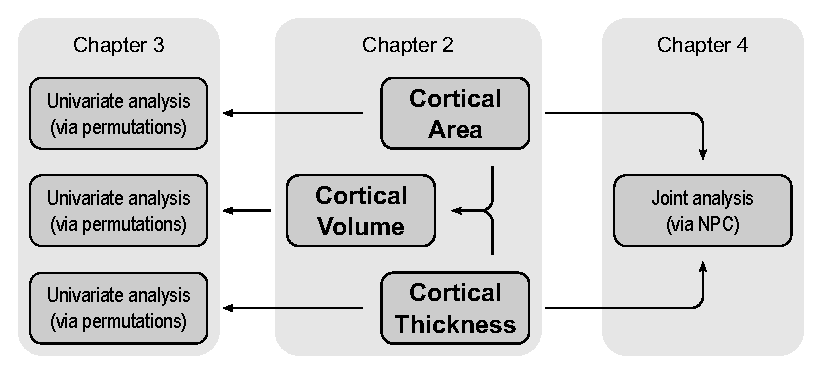
\includegraphics{images/flow.eps}}
\end{center}
\caption[Some possible analyses of cortical morphometric measurements using permutation tests.]{Some possible analyses of cortical morphometric measurements using permutation tests. Inter-subject comparisons of cortical area and other areal quantities, such as volume, that depends on both area and thickness, use the methods proposed in Chapter~\ref{sec:areal}. Univariate statistical analysis of each of these separately use the strategy discussed in Chapter~\ref{sec:perm}. Joint (combined) analysis of area and thickness, that bypass volumes altogether, use the methods proposed in Chapter~\ref{sec:comb}, in particular the non-parametric combination (\textsc{npc}), but also classical multivariate tests.}
\label{fig:intro:flow}
\end{figure}

\section{Methods for areal quantities}

The general strategy for analyses of cortical measurements consists of the generation of a surface-representation of the brain and its subsequent transformation into a sphere. Vertices of this sphere are then shifted along its surface to allow alignment that matches some feature of interest, such as sulcal depth, myelin content, or functional markers. As the alignment is performed, quantities assigned to vertices or faces, such as thickness or area, are carried along these vertices and faces. Once registration is done, these quantities are interpolated to a common grid (mesh), where comparisons between subjects can be performed.  

While methods to study thickness across subjects are available \citep{Fischl2000}, and use interpolation to a common reference grid using methods such as nearest neighbour or barycentric, such interpolation strategies cannot be used for either cortical area itself, nor to other areal quantities, such as cortical volume, as these are not mass-conservative (pycnophylactic). Chapter~\ref{sec:areal} clarifies the distinction between the nature of these measurements, and proposes the use of areal interpolation. This strategy permits quantities to be studied in absolute terms, as opposed to relative to some reference brain. The chapter proposes that areal quantities are analysed directly in the faces of the mesh from which they were computed, instead of resampled to vertices, which halves the resolution.

We demonstrate that areal data do not follow a normal distribution, being better characterised by a mixture of normal and lognormal distributions, in proportions that vary across the brain and possibly according to the scale of measurement. A power transformation can be considered to address lognormality, although a better alternative is to use permutation methods, that not only do not rely on distributional assumptions, but also allow correction for multiple testing and the use of non-standard statistics.

\section{Methods for permutation inference}

Permutation methods can provide exact control of false positives, making only weak assumptions about the data, and have been available in brain imaging for many particular cases \citep{Holmes1996, Nichols2002}, although no implementation for surface-based methods, even less so for facewise data as we have developed, existed in the literature until this work. With the recent availability of fast and inexpensive computing, the main limitation of permutation tests would be a certain lack of flexibility with respect to arbitrary experimental designs, in particular with respect to nuisance variables in the model, as well as repeated measurements. 

In Chapter~\ref{sec:perm} we report on results on approximate permutation strategies that are more flexible with respect to experimental designs that include such nuisances. We review the literature and conduct detailed simulations to identify the best method for settings that are typical for imaging research. A generic framework for permutation inference for complex general linear models (\textsc{glm}s) when the errors are exchangeable and/or have a symmetric distribution, is presented. Even in the presence of nuisance effects, these permutation inferences are powerful and provide control of false positives in a wide range of common and relevant imaging research scenarios.

We also demonstrate how the inference on \textsc{glm} parameters, originally intended for independent data, can be used in certain special but useful cases in which independence is violated, by means of using exchangeability blocks, that is, sets of observations with shared non-independence, and that can sometimes be treated as a single unit for permutation, i.e., shuffled as a whole, or sometimes serve as delimiters such that permutations happen only within block. The definition of exchangeability blocks allow for groups of observations with same variances, either known or assumed, thus requiring a statistic that preserves certain desirable properties for control of multiple testing even under such scenarios. We provide such a statistic, dubbed $G$-statistic, which is a generalisation of the $F$-statistic, as well as others.

\section{Methods for joint permutation inference}

While gray matter volume can be studied directly using the methods discussed in Chapter~\ref{sec:areal}, it may be the case that true effects affecting thickness and area in opposite directions may cancel each other out. Yet, analysing them separately using univariate methods as in Chapter~\ref{sec:perm} may not aggregate power from having effects acting the two simultaneously. Likewise, participants of an imaging study are often subjected to the acquisition of more than one imaging modality. These modalities are often analysed separately. However, a joint analysis have potential to answer more complex questions and to increment power. Moreover, even a single modality can sometimes be partitioned into subcomponents that disentangle different aspects of brain structure or function. Examples include independent component analysis, as well as scalar measurements from diffusion-tensor imaging. 

In Chapter~\ref{sec:comb} we show how permutation methods can be applied to combination analyses such as those that include multiple imaging modalities, multiple data acquisitions of the same modality, or simply multiple hypotheses on the same data. Using the well-known definition of union-intersection tests and closed testing procedures, we use synchronised permutations to correct for such multiplicity of tests, allowing flexibility to integrate imaging data with different spatial resolutions, surface and/or volume-based representations of the brain, including non-imaging data. 

In particular for the problem of joint inference, we propose and evaluate a modification of the recently introduced Non-Parametric Combination (\textsc{npc}) methodology \citep{Pesarin2010}, such that instead of a two-phase algorithm and large data storage requirements, the inference can be performed in a single phase, with reasonable computational demands. We also evaluate, in the context of permutation tests, various combining methods that have been proposed in the past decades, and identify those that provide the best control over error rate and power across a range of situations. We show that one of these, the method of \citet{Tippett1931}, provides a link between correction for the multiplicity of tests and their combination.

Finally, we discuss how the correction can solve certain problems of multiple comparisons in common designs, and how the combination is distinguished from conjunctions, even though both can be assessed using permutation tests. We also provide a common algorithm that accommodates combination and correction.
\cleardoublepage \chapter{Areal quantities in the cortex}
\label{sec:areal}
\setstretch{\lspac}

\section{Introduction}

The surface area of the cerebral cortex greatly differs across species, whereas the cortical thickness has remained relatively constant during evolution \citep{Mountcastle1998, Fish2008}. At a microanatomic scale, regional morphology is closely related to functional specialization \citep{Roland1998, Zilles2010}, contrasting with the columnar organization of the cortex, in which cells from different layers respond to the same stimulus \citep{EGJones2000, Buxhoeveden2002}. In addition, \citet{Rakic1988} proposed an ontogenetic model that explains the processes that lead to cortical arealization and differentiation of cortical layers according to related, yet independent mechanisms. Supporting evidence for this model has been found in studies with both rodent and primates, including humans \citep{Chenn2002, Rakic2009}, as well as in pathological states \citep{Rimol2010b, Bilguvar2010}.

At least some of the variability of the distinct genetic and developmental processes that seem to determine regional cortical area and thickness can be captured using polygon mesh (surface-based) representations of the cortex derived from $T_1$-weighted magnetic resonance imaging (\textsc{mri}) \citep{Panizzon2009, Winkler2010, SanabriaDiaz2010}. In contrast, volumetric (voxel-based) representations, also derived from \textsc{mri}, were shown to be unable to readily disentangle these processes \citep{Winkler2010}. Figure~\ref{fig:areal:geometry} shows schematically the difference between these two representations.

\begin{figure}[!tp]
\centering
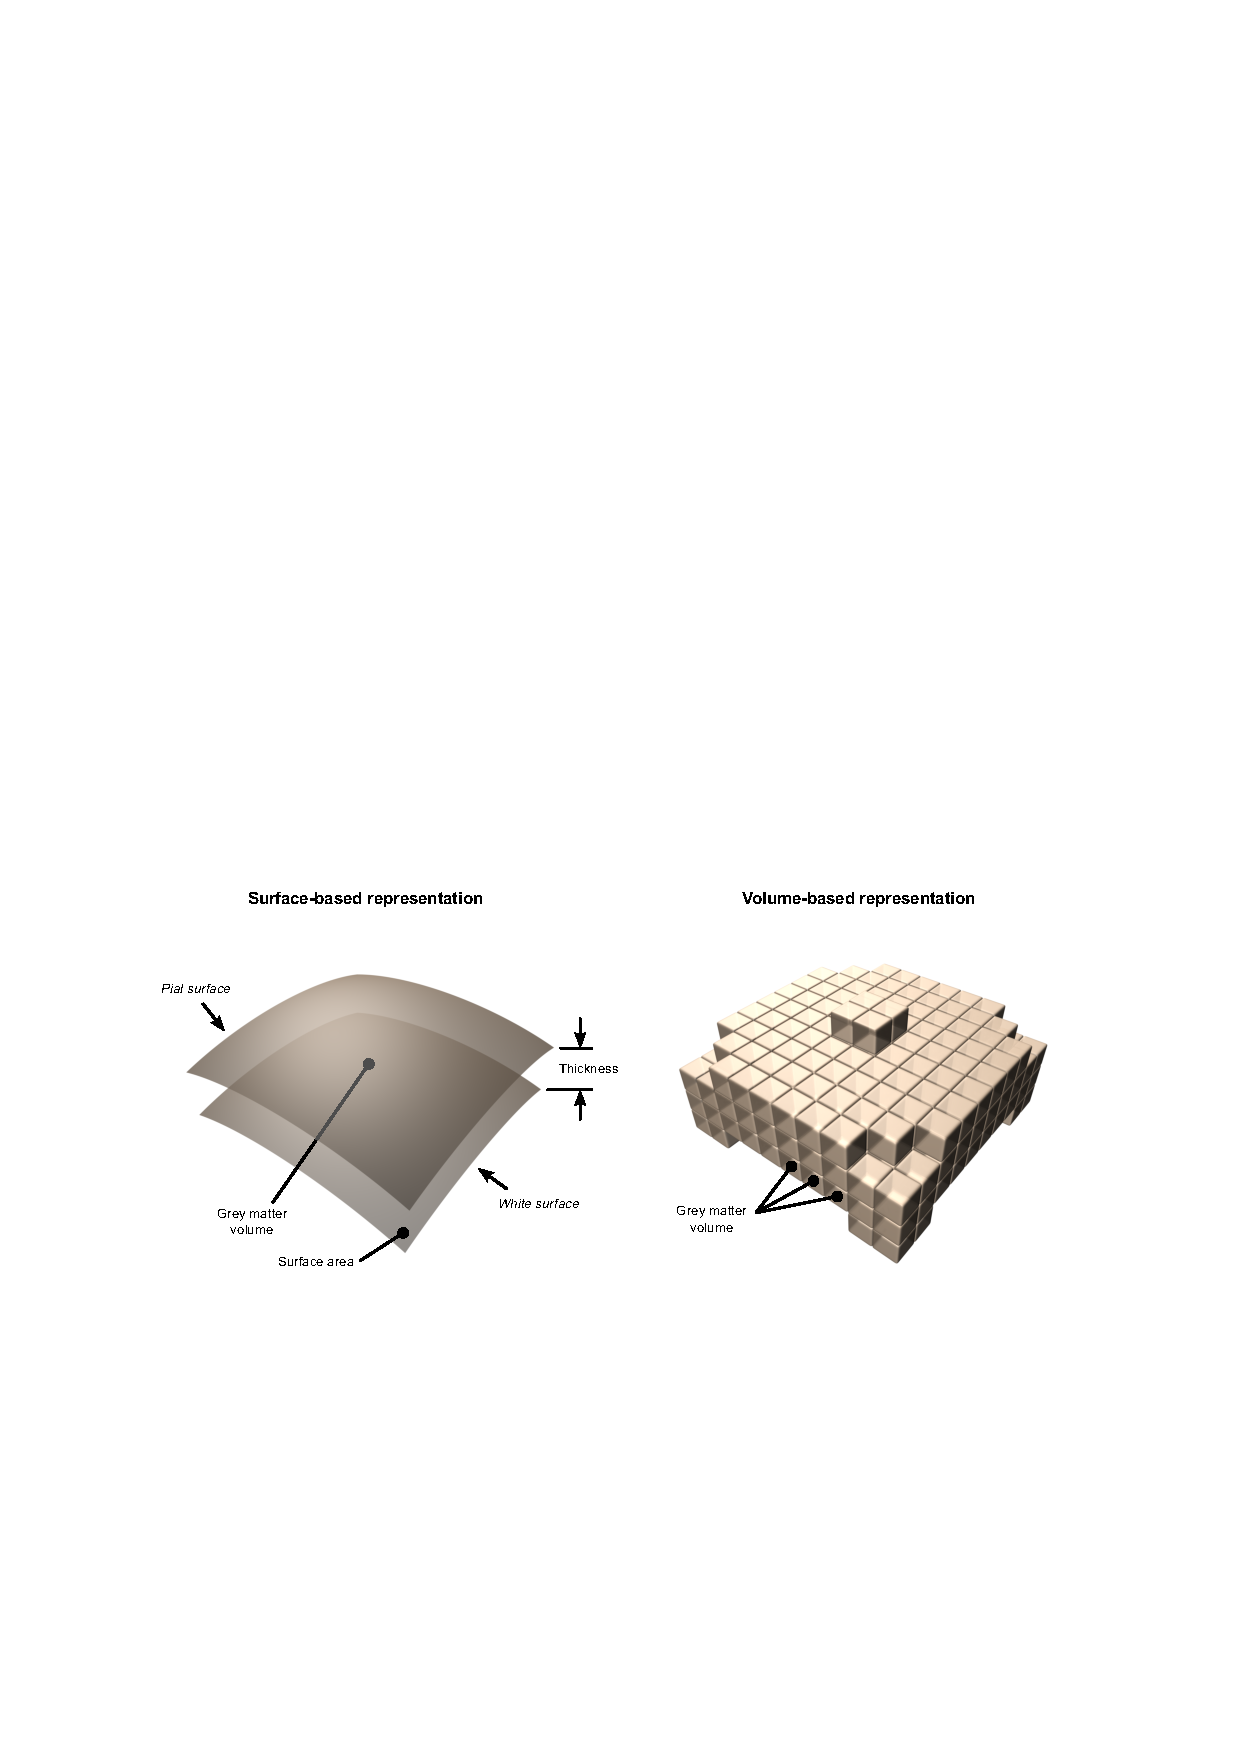
\includegraphics[width=14cm]{images/geometry.jpg}
\caption[Surface- and volume-based representations of the cortex.]{Geometrical relationship between cortical thickness, surface area and grey matter volume. In the surface-based representation, the grey matter volume is a quadratic function of distances in the surfaces and a linear function of the thickness. In the volume-based representation, only the volumes can be measured directly and require partial volume-effects to be considered \citep{Winkler2010}.}
\label{fig:areal:geometry}
\end{figure}

Mesh representations of the brain allow measurements of the cortical thickness at every point in the cortex, as well as estimation of the average thickness for pre-specified regions. However, to date, analyses of cortical surface area have been generally limited to two types of studies: (1) vertexwise comparisons with a standard brain, using some kind of expansion or contraction measurement, either of the surface itself \citep{Joyner2009, Lyttelton2009, Hill2010, Rimol2010b, Palaniyappan2011}, of linear distances between points in the brain \citep{Sun2009a, Sun2009}, or of geometric distortion \citep{Wisco2007}, or (2) analyses of the area of regions of interest (\textsc{roi}) defined from postulated hypotheses or from macroscopic morphological landmarks \citep{Dickerson2009, Nopoulos2010, Kahler2011, Durazzo2011, Schwarzkopf2011, Eyler2011, Chen2011_neuron, Chen2012}. Analyses of expansion, however, do not deal with area directly, depending instead on non-linear functions associated with the warp to match the standard brain, such as the Jacobian of the transformation. Moreover, by not quantifying the amount of area, these analyses are only interpretable with respect to the brain used for the comparisons. R\textsc{oi}-based analyses, on the other hand, entail the assumption that each region is homogeneous with regard to the feature under study, and have maximum sensitivity only when the effect of interest is present throughout the \textsc{roi}.

These difficulties can be obviated by analysing each point on the cortical surface of the mesh representation, a method already well established for cortical thickness \citep{Fischl2000}. Pointwise measurements, such as thickness, are generally taken at and assigned to each vertex of the mesh representation of the cortex. This kind of measurement can be transferred to a common grid and subjected to statistical analysis. Standard interpolation techniques, such as nearest neighbor, barycentric \citep{Yiu2000}, spline-based \citep{DeBoor1962} or distance-weighted \citep{Shepard1968} can be used for this purpose. The resampled data can be further spatially smoothed to alleviate residual interpolation errors. However, this approach is not suitable for areal measurements, since area is not inherently a point feature. To illustrate this aspect, an example is given in Figure~\ref{fig:areal:forest}. Methods that can be used for interpolation of point features do not necessarily compensate for inclusion or removal of datapoints,\footnote{A notable exception is the natural neighbor method \citep{Sibson1981}. However, the original method needs modification for use with areal analyses.} unduly increasing or reducing the global or regional sum of the quantities under study, precluding them for use with measurements that are, by nature, areal. The main contribution of this chapter is to address the technical difficulties in analysing the local brain surface area, \emph{as well as any other cortical quantity that is areal by nature}. We propose a framework to analyse areal quantities and argue that a mass preserving interpolation method is a necessary step. We also study different processing strategies and characterize the distribution of \emph{facewise} cortical surface area.

\begin{figure}[!p]  % Figure 1
\centering
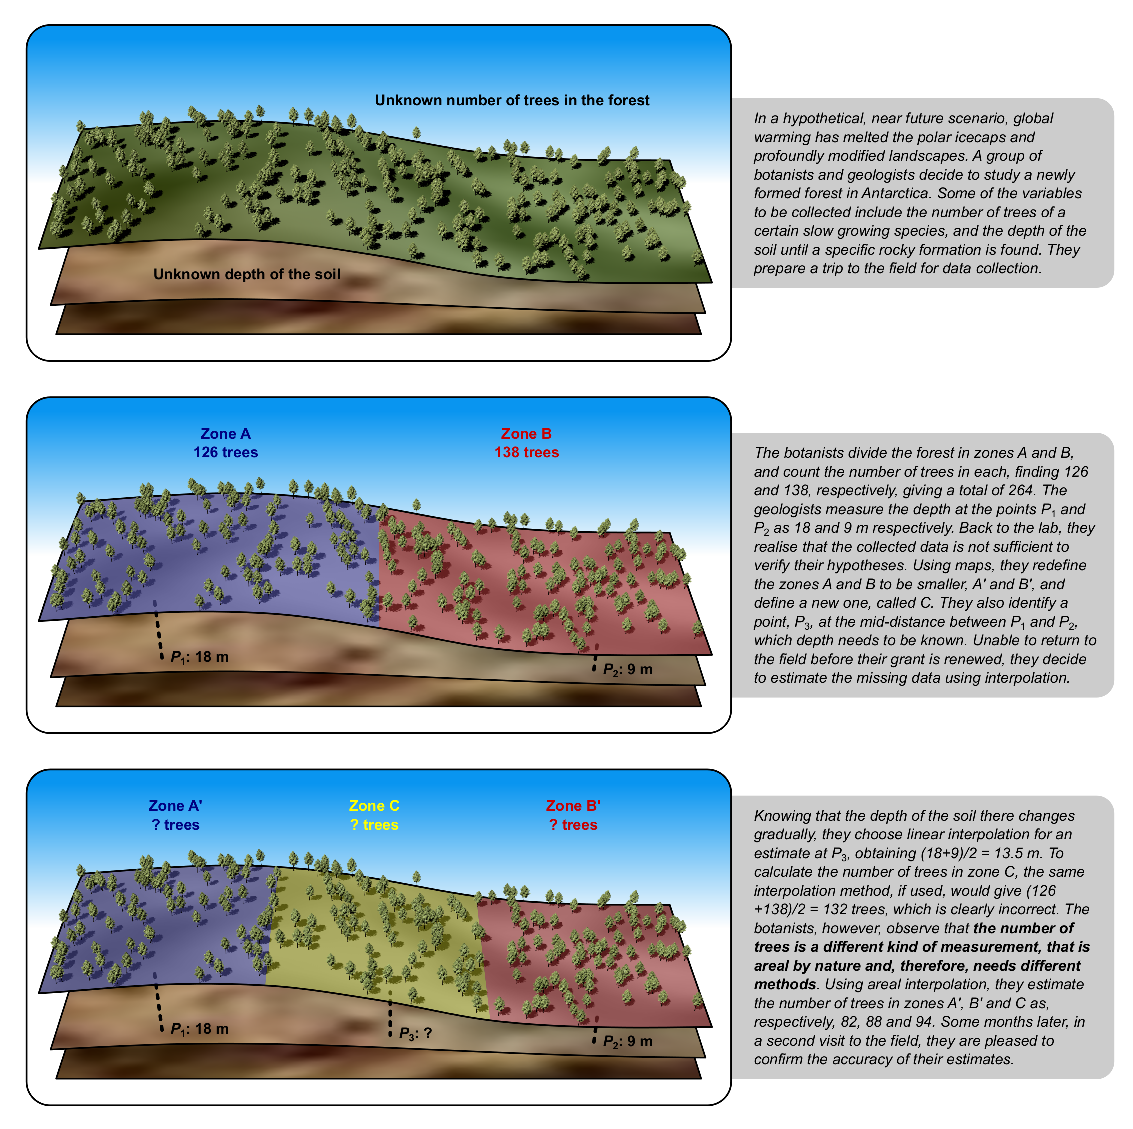
\includegraphics[width=14cm]{images/forest.eps}
\caption[Example demonstrating differences between area and point measurements.]{An example demonstrating differences in the nature of measurements. In this analogy, the depth of the soil is similar to brain cortical thickness, whereas the number of trees is similar to areal quantities distributed across the cortex. These areal quantities can be the surface area itself (in this case, the area of the terrain), but can also be any other measurement that is areal by nature (such as the number of trees).}
\label{fig:areal:forest}
\end{figure}

\section{Method}

An overview of the method is presented in Figure~\ref{fig:areal:overview}. Comparisons of cortical area between subjects require a surface model for the cortex to be constructed. A number of approaches are available \citep{Mangin1995, Dale1999, vanEssen2001, Kim2005} and, in principle, any could be used. Here we adopt the method of \citet{Dale1999} and \citet{Fischl1999_cortical}, as implemented in the FreeSurfer software package (\textsc{fs}).\footnote{Available at \href{http://surfer.nmr.mgh.harvard.edu}{http://surfer.nmr.mgh.harvard.edu}.} In this method, the $T_1$-weighted images are initially corrected for magnetic field inhomogeneities and skull-stripped \citep{Segonne2004}. The voxels belonging to the white matter (\textsc{wm}) are identified based on their locations, on their intensities, and on the intensities of the neighboring voxels. A mass of connected \textsc{wm} voxels is produced for each hemisphere, using a six-neighbors connectivity scheme, and a mesh of triangular faces is tightly built around this mass, using two triangles per exposed voxel face. The mesh is smoothed taking into account the local intensity in the original images \citep{Dale1993}, at a subvoxel resolution. Topological defects are corrected \citep{Fischl2001,Segonne2007} ensuring that the surface has the same topological properties of a sphere. A second iteration of smoothing is applied, resulting in a realistic representation of the interface between gray and white matter (the \emph{white surface}). The external cortical surface (the \emph{pial surface}), which corresponds to the pia mater, is produced by nudging outwards the white surface towards a point where the tissue contrast is maximal, maintaining constraints on its smoothness and on the possibility of self-intersection \citep{Fischl2000}. The white surface is inflated in an area-preserving transformation and subsequently homeomorphically transformed to a sphere \citep{Fischl1999_intersubject}. After the spherical transformation, there is a one-to-one mapping between faces and vertices of the surfaces in the native geometry (white and pial) and the sphere. These surfaces are comprised exclusively of triangular faces.

\begin{figure}[!p]  % Figure 2
\centering
\includegraphics[width=14cm]{images/overview.png}
\caption[Overview of areal analyses.]{Diagram of the steps to analyse the cortical surface area. For clarity, the colors represent the convexity of the surface, as measured in the native geometry.}
\label{fig:areal:overview}
\end{figure}

\subsection{Area per face and other areal quantities}

The surface area for analysis is computed at the interface between gray and white matter, i.e.\ at the \emph{white surface}. Another possible choice is to use the middle surface, i.e.\ a surface that runs at the mid-distance between white and pial. Although this surface is not guaranteed to match any specific cortical layer, it does not over or under-represent gyri or sulci \citep{vanEssen2005}, which might be an useful property. The white surface, on the other hand, matches directly a morphological feature and also tends to be less sensitive to cortical thinning or thickening than the middle or pial surfaces. Whenever methods to produce surfaces that represent biologically meaningful cortical layers are available, these should be preferred.

In contrast to conventional approaches in which the area of all faces that meet at a given vertex is summed and divided by three, producing a measure of the \emph{area per vertex}, for facewise analysis it is the \emph{area per face} that is measured and analysed. Since for each subject, each face in the native geometry has its corresponding face on the sphere, the value that represents area per face, as measured from the native geometry, can be mapped directly to the sphere, despite any areal distortion introduced by the spherical transformation.

Furthermore, since there is a direct mapping that is independent of the actual area in the native geometry, \emph{any other quantity that is biologically areal can also be mapped to the spherical surface}. Perhaps the most prominent example is cortical volume (Section~\ref{sec:areal:volumes}), although other cases of such quantities, that may potentially be better characterized as areal processes, are the extent of the neural activation as observed with functional \textsc{mri}, the amount of amyloid deposited in Alzheimer's disease \citep{Klunk2004, Clark2011}, or simply the the number of cells counted from optic microscopy images reconstructed to a tri-dimensional space \citep{Schormann1998}. Since areal interpolation (described below) conserves locally, regionally and globally the quantities under study, it allows accurate comparisons and analyses across subjects for measurements that are areal by nature, or that require mass conservation on the surface of the mesh representation.

\subsection{Computation of surface area}

The facewise areas in the mesh representation of the brain can be computed trivially: for a triangular face $ABC$ with vertices $\mathbf{a}=[x_A \; y_A \; z_A]'$, $\mathbf{b}=[x_B \; y_B \; z_B]'$, and $\mathbf{c}=[x_C \; y_C \; z_C]'$, the area is $|\mathbf{u} \times \mathbf{v}|/2$, where $\mathbf{u} = \mathbf{a}-\mathbf{c}$, $\mathbf{v} = \mathbf{b}-\mathbf{c}$, $\times$ represents the cross product, and $|\bullet|$ represents the vector norm.

\subsection{Volume as an areal quantity}
\label{sec:areal:volumes}

Gray matter volume can be assessed using the partial volume effects of the gray matter in a per-voxel fashion using volume-based representations of the brain, such as in voxel-based morphometry \citep[\textsc{vbm}][]{Ashburner2000}, or as the amount of tissue present between the gray and white surfaces in surface-based representations. Using the surface-based representation, software such as FreeSurfer up to version 5.3.0 compute the volume through the following steps:

\begin{enumerate}
\item The area at each vertex is computed as $\sfrac{1}{3}$ of the sum of the areas of all faces of the white surface that have that vertex in common. 
\item The volume is computed as the product of the area by the thickness at that vertex.
\end{enumerate}

This procedure, while providing a good approximation that is already superior to volume-based measurements for not being as susceptible to various artefacts that can affect the latter \citep{Ashburner2009}, is still problematic. Simple multiplication of thickness by area leaves considerable amounts of tissue unmeasured at the gyri, while measuring more than once pieces of tissue in the fundi of sulci. Figure~\ref{fig:areal:mantle} shows a simplification to a two-dimensional case of this phenomenon, that affects differentially, and in opposite directions, sulci and gyri.

\begin{figure}[!tp]
\centering
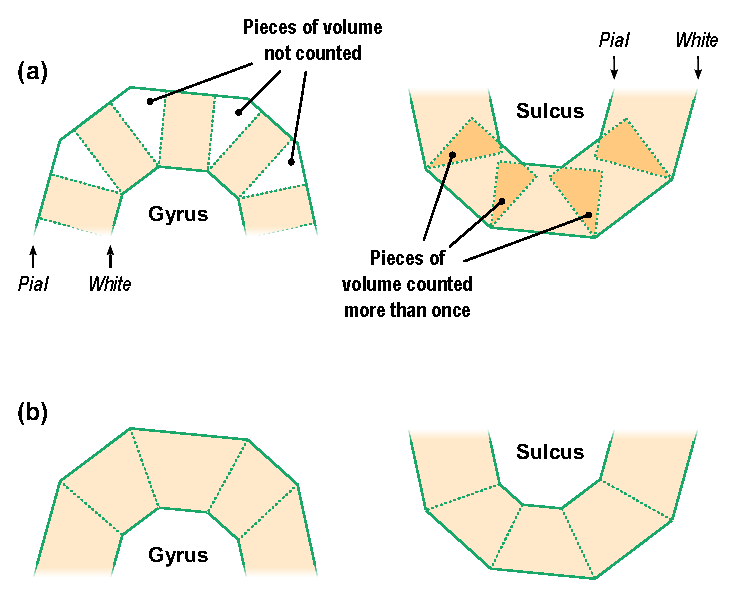
\includegraphics{images/mantle.eps}
\caption[Simple multiplication leaves tissue over- or under-represented.]{(\emph{a}) A simplified two-dimensional representation of the cortex. If the volume is computed using simple multiplication of thickness by area, considerable amount of tissue is left unmeasured in the gyri, or measured more than once in sulci. (\emph{b}) The proposed method, would compute analytically the volumes of the regions of tissue between matching faces of white and pial surfaces, leaving no part of tissue unmeasured.}
\label{fig:areal:mantle}
\end{figure}

The problem can be alleviated to some extent by using the mid-surface as the reference for area, as opposed to the white. Instead, a more exact solution is proposed here. It consists of using the three vertices that define a face in the white surface, and the matching vertices in the pial surface, to define an \emph{oblique truncated triangular pyramid}, which on its turn can be perfectly subdivided into three non-overlapping tetrahedra; the volumes of these are computed analytically, summed and assigned to each face of the surface representation, and used for subsequent analysis. Figure~\ref{fig:areal:pyramid} illustrates the procedure. More specifically, the procedure is as follows:

\begin{figure}[!tp]
\centering
\includegraphics[width=14cm]{images/pyramid.eps}
\caption[Proposed method to compute volumes in the cortex.]{(\emph{a}) In the surface representation, the cortex is limited internally by the white and externally by the pial surface. (\emph{b}) and (\emph{c}) These two surfaces have matching vertices that can be used to delineate an oblique truncated triangular pyramid. (\emph{d}) In the proposed method, the six vertices of this pyramid are used to define three tetrahedra, the volumes of which are computed analytically.}
\label{fig:areal:pyramid}
\end{figure}

\begin{enumerate}
\item For a given face $A_w B_w C_w$ in the white surface, and its corresponding face $A_p B_p C_p$ in the pial surface, define an oblique truncated triangular pyramid using these six vertices.
\item Split this truncated pyramid into three tetrahedra: $T_1 = (A_w,B_w,C_w,A_p)$, $T_2 = (A_p,B_p,C_p,B_w)$, and $T_3 = (A_p,C_p,C_w,B_w)$.
\item For each such tetrahedra, let $\mathbf{a}$, $\mathbf{b}$, $\mathbf{c}$ and $\mathbf{d}$ represent its four vertices in terms of coordinates $[x\;y\;z]'$. Compute the volume as $|\mathbf{u}\cdot(\mathbf{v} \times \mathbf{w})|/6$, where $\mathbf{u} = \mathbf{a}-\mathbf{d}$, $\mathbf{v} = \mathbf{b}-\mathbf{d}$, $\mathbf{w} = \mathbf{c}-\mathbf{d}$, $\times$ represents the cross product, $\cdot$ represents the dot product, and $|\bullet|$ represents the vector norm.
\end{enumerate}

The procedure can be accelerated by setting $\mathbf{d}=A_p$, that is, the common vertex for all three tetrahedra, such that the vector subtractions can happen only once for all three. If vertexwise values are needed, these can be computed as $\sfrac{1}{3}$ of the volumes of all faces that meet at that vertex.

\subsection{Registration}

Registration to a common coordinate system is necessary to allow comparisons across subjects \citep{Drury1996}. The registration is performed by shifting vertex positions along the surface of the sphere until there is a good alignment between subject and template (target) spheres with respect to certain specific features, usually, but not necessarily, the cortical folding patterns. As the vertices move, the areal quantities assigned to the corresponding faces are also moved along the surface. The target for registration should be the less biased as possible in relation to the population under study \citep{Thompson2002}.

A registration method that produces a smooth, i.e.\ spatially differentiable, warp function enables the smooth transfer of areal quantities. A possible way to accomplish this is by using registration methods that are diffeomorphic. A diffeomorphism is an invertible transformation that has the elegant property that it and its inverse are both continuously differentiable \citep{Christensen1996, Miller1997}, minimising the risk of vagaries that would be introduced by the non-differentiability of the warp function.

Diffeomorphic methods are available for spherical meshes \citep{Glaunes2004, Yeo2010, Robinson2014}, and here we adopt the Spherical Demons (\textsc{sd}) algorithm\footnote{Available at \href{http://sites.google.com/site/yeoyeo02/software/sphericaldemonsrelease}{http://sites.google.com/site/yeoyeo02/software/sphericaldemonsrelease}.} \citep{Yeo2010}. \textsc{Sd} extends the Diffeomorphic Demons algorithm \citep{Vercauteren2009} to spherical surfaces. The Diffeomorphic Demons algorithm is a diffeomorphic variant of the efficient, non-parametric Demons registration algorithm \citep{Thirion1998}. \textsc{Sd} exploits spherical vector spline interpolation theory and efficiently approximates the regularization of the Demons objective function via spherical iterative smooting.

Methods that are not diffeomorphic by construction \citep{Fischl1999_intersubject, Auzias2013}, but in practice produce invertible and smooth warps could, in principle, be used for registration for areal analyses. In the Evaluation section we study the performance of different registration strategies as well as the impact of the choice of the template.

\subsection{Areal interpolation}

After the registration, the correspondence between each face on the registered sphere and each face from the native geometry is maintained, and the surface area or other areal quantity under study can be transferred to a common grid, where statistical comparisons between subjects can be performed. The common grid is a mesh which vertices lie on the surface of a sphere. A geodesic sphere, which can be constructed by iterative subdivision of the faces of a regular icosahedron, has many advantages for this purpose, namely, ease of computation, edges of roughly similar sizes and, if the resolution is fine enough, edge lengths that are much smaller than the diameter of the sphere (see Section~\ref{sec:areal:geosphere} for details). These two spheres, i.e.\ the registered, irregular spherical mesh (source), and the common grid (target), typically have different resolutions. The interpolation method must, nevertheless, \emph{conserve the areal quantities}, globally, regionally and locally. In other words, the method has to be \emph{pycnophylactic}\footnote{From Greek \emph{pyknos} = mass, density, and \emph{phylaxis} = guard, protect, preserve, meaning that the method has to be mass conservative.} \citep{Tobler1979}. This is accomplished by assigning, to each face in the target sphere, the areal quantity of all overlapping faces from the source sphere, weighted by the fraction of overlap between them (Figure~\ref{fig:areal:triangles}).

\begin{figure}[!t]  % Figure 3
\centering
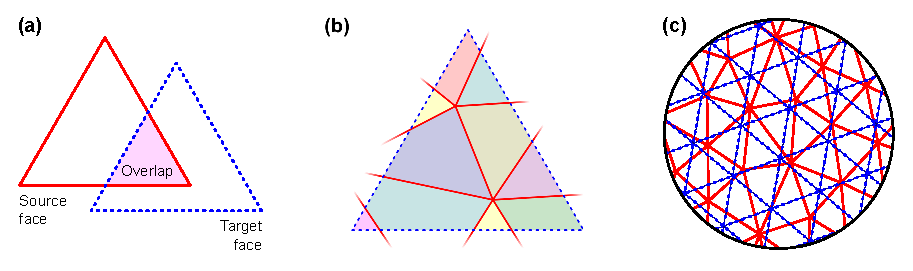
\includegraphics[width=14cm]{images/triangles.eps}
\caption[Overlapping areas used to weight areal quantities during interpolation.]{(\emph{a}) Areal interpolation between a source and a target face uses the overlapping area as a weighting factor. (\emph{b}) For a given target face, each overlapping source face contributes an amount of areal quantity. This amount is determined by the proportion between each overlapping area (represented in different colors) and the area of the respective source face. (\emph{c}) The interpolation is performed at multiple faces of the target surface, so that the amount of areal quantity assigned to a given source face is conservatively redistributed across one or more target faces.}
\label{fig:areal:triangles}
\end{figure}

More specifically, let $Q^{S}_{i}$ represent the areal quantity on the $i$-th face of the registered, source sphere $S$, $i=1,2,\ldots,I$. This areal quantity can be directly mapped back to the native geometry, and can be the area per face as measured in the native geometry, or any other quantity of interest that is areal by nature. Let the actual area of the same face on the source sphere be indicated by $A^{S}_{i}$. The quantities $Q^{S}_{i}$ have to be transfered to a target sphere $T$, the common grid, which face areas are given by $A^{T}_{j}$ for the $j$-th face, $j=1,2,\ldots,J$, $J \neq I$. Each target face $j$ overlaps with $K$ faces of the source sphere, being these overlapping faces indicated by indices $k=1,2,\ldots,K$, and the area of each overlap indicated by $A^{O}_{k}$. The interpolated areal quantity to be assigned to the $j$-th target face is then given by:

\begin{equation}
Q^{T}_{j} = \sum_{k=1}^{K} \frac{A^{O}_{k}}{A^{S}_{k}} Q^{S}_{k}
\end{equation}

Similar interpolation schemes have been devised to solve problems in geographic information systems (\textsc{gis}) \citep{Markoff1973, Goodchild1980, Flowerdew1991, Gregory2010}. Surface models of the brain impose at least one additional challenge, which we address in the implementation (see Section~\ref{sec:areal:implementation}). Differently than in other fields, where interpolation is performed over geographic territories that are small compared to Earth and, therefore, can be projected to a plane with acceptable areal distortion, here we have to interpolate across the whole sphere. Although other conservative interpolation methods exist for this purpose \citep{Jones1999, Lauritzen2008, Ullrich2009}, these methods either use regular latitude-longitude grids, cubed-spheres, or require a special treatment of points located above a certain latitude threshold to avoid singularities at the poles. These disadvantages may render these methods suboptimal for direct use in brain imaging.

\subsection{Implementation}
\label{sec:areal:implementation}

The areal interpolation for spheres is implemented in two parts. In the first, we compute inside of which source faces the target vertices are located, creating a lookup table to be used in the second part. This is the point-in-polygon problem found in vector graphics applications \citep{Vince2005}. Here we calculate the area of each source face, $A^{S}_{i}$, and the subsequent steps proceed iteratively for each face in the source. The barycentric coordinates of each candidate vertex in relation to the current face $i$ is computed; if their sum equals to unity, the point is labelled as inside. However, to test if all vertices are inside every face would needlessly waste computational time. Moreover, since all points are on the surface of a sphere, the vertices in the target are never expected to be coplanar to the source triangular faces, so the test would always fail. The first problem is treated by testing only the vertices located within a bounding box defined, still in the \textsc{3d} space, from the source face extreme coordinates. The second could na\"{i}vely be treated by converting the \textsc{3d} Cartesian coordinates to \textsc{2d} spherical coordinates, which allow a fast flattening of the sphere to the popular plate carr\'{e}e cylindrical projection. However, latitude is ill-defined at the poles in cylindrical projections. Moreover, cylindrical projections introduce a specific type of deformation that is undesired here: straight lines on the surface (geodesic lines) are distorted. The solution we adopt is to rotate the Cartesian coordinate system so that the barycenter of the current source face lies at the point $[r\;0\;0]'$, where $r$ is the radius of the source and target spheres. The barycenter is used for ease of calculation and for being always inside the triangle. After rotation, the current face and the nearby candidate target vertices are projected to a plane using the azimuthal gnomonic projection \citep{Snyder1987}, centered at the barycenter of the face. The point-in-polygon test can then be applied successfully. The key advantage of the gnomonic projection is that all geodesics project as straight lines, rather than loxodromic or other complex paths as with other projections, which would cause many target vertices to be incorrectly labelled. This projection can be obtained trivially after the rotation of the \textsc{3d} Cartesian coordinate system as $\phi=y/x$ and $\theta=z/x$, where $[x\;y\;z]'$ are the \textsc{3d} coordinates of the point being projected. A potential disadvantage of the gnomonic projection is the remarkable areal distortion for regions distant from the center of the projection. Since in typical neuroimaging applications the source and target spheres are composed of a tessellation of approximately $3\times10^6$ faces, $A^{S}_{i} \ll 4 \pi r^2$, and the distortion becomes negligible.

In the second part, the areal interpolation is performed, with the overlapping areas being calculated and used to weigh the areal quantity under study. The identification of intersections between two sets of polygons is also a well studied problem in vector graphics \citep{Guibas1987, Chazelle1994}, which solution depends on optimally finding crossings between multiple line segments \citep{Bentley1979, Chazelle1992, Balaban1995}. Most of the efficient available algorithms assume that the polygons are all coplanar; those that work in the surface of a sphere use coordinates expressed in latitude and longitude and require special treatment of the polar regions. The solution we adopt obviates these problems by first computing the area of each target face, $A^{T}_{j}$; the subsequent steps are performed iteratively for each face in the target sphere, using the azimuthal gnomonic projection, similarly as in the first part, but now centered at the barycenter of the current target face at every iteration. The areal quantities assigned to the faces in the target sphere are initialized as zero before the loop begins. If all three vertices of the current target face $j$ lie inside the same source face $k$, as known from the lookup table produced in the first part, then to the current face the areal quantity given by $Q^{T}_{j} = Q^{S}_{k} A^{T}_{j} / A^{S}_{k}$ is assigned. Otherwise, the source faces that surround the target are examined to find overlaps. This is done by considering the edges of the current target face as vectors organised in counter-clockwise orientation, and testing if the vertices of the candidate faces lie on the left, right or if they coincide with the edge. If all the three vertices of any candidate face are on the right of any edge, there is no overlap and the candidate face is removed from further consideration. If all the three vertices are on the left of all three edges, then the candidate source face is entirely inside the target, which has then its areal quantity incremented as $Q^{T}_{j} \leftarrow Q^{T}_{j} + Q^{S}_{k}$. The remaining faces are those that contain some vertices on the left and some on the right of the edges of the current, target face. The intersections between these source and target edges are computed and false intersections between edge extensions are ignored. A list containing the vertices for each candidate source face that are inside the target face (known for being on the left of the three target edges), the target vertices that are inside each of the source faces (known from the lookup table) and the coordinates of the intersections between face edges, is used to compute the convex hull, using the Quickhull algorithm \citep{Barber1996}. The convex hull delimits the overlapping region between the current target face $j$ and the candidate source face $k$, which area, $A^{O}_{k}$, is used to increment the areal quantity assigned to the target face as $Q^{T}_{j} \leftarrow Q^{T}_{j} + Q^{S}_{k} A^{O}_{k}/A^{S}_{k}$.

The algorithm runs in $\mathcal{O}(n)$ for $n$ faces, as opposed to $\mathcal{O}(n^2)$ that would be obtained by na\"ive search. Nevertheless, the current implementation, that runs in Octave \citep{Eaton2015} or \textsc{matlab} \citep{MATLAB2015}, a dynamically typed, interpreted language, requires about 24 hours to run in a computer with 2.66~GHz Intel Xeon processors.


\subsection{Geodesic spheres and areal inequalities}
\label{sec:areal:geosphere}

The only required feature for the common grid used for the areal interpolation is that all its vertices must lie on the surface of a sphere. The algorithm we present in Section~\ref{sec:areal:implementation} requires further that all faces of the sphere are triangular and that all edges of all faces are much smaller than the radius, so that areal distortion is minimised when projecting to a plane.

A common grid that meet these demands is a sufficiently fine geodesic sphere. There are different ways to construct such a sphere \citep{Kenner1976}. One method is to subdivide each face of a regular polyhedron with triangular faces, such as the icosahedron, into four new triangles. The new vertices are projected to the surface of the (virtual) circumscribed sphere along its radius and the process is repeated recursively a number of times \citep{Lauchner1969}. For the $n$-th iteration, the number of faces is given by $F=4^nF_0$, the number of vertices by $V=4^n(V_0-2)+2$, and the number of edges by $E=4^nE_0$, where $F_0$, $V_0$ and $E_0$ are, respectively, the number of faces, vertices and edges of the polyhedron with triangular faces used for the initial subdivision. For the icosahedron, $F_0=20$, $V_0=12$ and $E_0=30$ (Figure~\ref{fig:areal:geosphere}\emph{a}). For the analyses in this manuscript, we used $n=7$, producing geodesic spheres with 327680 faces and 163842 vertices.

These faces, however, do not have identical edge lengths and areas \citep{Kenner1976}, even though the initial icosahedron was perfectly regular. This is important for areal interpolation, as larger faces on the target grid do overlap with more faces from the source surfaces, absorbing larger amounts of areal quantities, possibly causing confusion if one attempts to color-encode the interpolated image according to the actual areal quantities, in which case, geometric patterns such as in Figure~\ref{fig:areal:geosphere}\emph{b} will become evident. Moreover, smoothing can cause quantities that are arbitrarily large or small due to face sizes to be blurred into the neighbors. Both potential problems can be addressed by multiplying the areal quantity at each face $j$, after interpolation, by a constant given by $4 \pi r^2/(A^{T}_{j}F)$, where $A^{T}_{j}$ is the area of the same face of the geodesic sphere, $F$ is the number of faces, and $r$ is the radius of the sphere.

\begin{figure}[!t]  % Figure 11
\centering
\includegraphics[width=14cm]{images/geosphere.png}
\caption[Geodesic spheres.]{(\emph{a}) The common grid can be a geodesic sphere produced from recursive subdivision of a regular icosahedron. At each iteration, the number of faces is quadruplied. (\emph{b}) After the first iteration, however, the faces no longer have regular sizes, with the largest face being approximately 1.3 times larger than the smallest as $n$ increases.}
\label{fig:areal:geosphere}
\end{figure}

\subsection{Smoothing}
\label{sec:areal:smoothing}

Smoothing can be applied to alleviate residual discontinuities in the interpolated data due to unfavorable geometric configurations between faces of source and target spheres. For the purpose of smoothing, facewise data can be represented either by their barycenters, or converted to vertexwise (see Section~\ref{sec:areal:presentation} for a discussion on how to convert), and should take into account differences on face sizes, as larger faces will tend to absorb more areal quantities (see Section~\ref{sec:areal:geosphere}). Smoothing can be applied using the moving weights method \citep{Lombardi2002}, defined as

\begin{equation}
\tilde{Q}^{T}_n = \frac{\sum_j Q^{T}_j G(g(\mathbf{x}_n,\mathbf{x}_j))}{\sum_j G(g(\mathbf{x}_n,\mathbf{x}_j))}
\end{equation}

\noindent where $\tilde{Q}^{T}_n$ is the smoothed areal quantity at the $n$-th face, $Q^{T}_j$ is the areal quantity assigned to each of the $J$ faces of the same surface before smoothing, $g(\mathbf{x}_n,\mathbf{x}_j)$ is the scalar-valued distance along the surface between the barycenter $\mathbf{x}_n$ of the current face and the barycenter $\mathbf{x}_j$ of another face, and $G(g)$ is the Gaussian kernel.\footnote{As with other neuroimaging applications, smoothing after registration implies that the effective filter width is not spatially constant in native space, neither is the same across subjects. Smoothing on the sphere also contributes to different filter widths across space due to the deformation during spherical transformation.}

\subsection{Conversion from facewise to vertexwise}
\label{sec:areal:conversion}

Whenever it is necessary to perform analyses that include measurements taken at each vertex (such as some areal quantity versus cortical thickness) or when only software that can display vertexwise data is available (Section~\ref{sec:areal:presentation}, it may be necessary to convert the areal quantities from facewise to vertexwise. The conversion can be done by redistributing the quantities at each face to their three constituent vertices. The areal values assigned to the faces that meet at a given vertex are summed, and divided by three, and reassigned to this vertex. Importantly, this procedure has to be done \emph{after} the areal interpolation, since interpolation methods for vertexwise data are not appropriate for areal quantities, and \emph{before} the statistical analysis, since the average of the results of the statistics of a test is not necessarily the same as the statistic for the average of the original data. It should also be observed that conversion from facewise to vertexwise data implies a loss of resolution to approximately half of the original and, therefore, should be performed only if resolution is not a concern and there is no other way to analyse, visualize, or present facewise data or results. The conversion does not change the underlying distribution, provided that the resolution of the initial mesh is sufficiently fine.

\subsection{Statistical analysis}

After resampling to a common grid, the facewise data is ready for statistical analysis. The most straightforward method is to use the general linear model (\textsc{glm}). The \textsc{glm} is based on a number of assumptions, including that the observed values have a linear, additive structure, that the residuals of the model fit have the same variance and are normally distributed. When these assumptions are not met, a non-linear transformation can be applied, as long as the true, biological or physical meaning that underlies the observed data is preserved. In the Evaluation section, we show empirically that facewise cortical surface area is largely not normal. Instead, the distribution is skewed and can be better characterized as \emph{lognormal}. A generic framework that can accommodate arbitrary areal quantities with skewed distributions is using a power transformation, such as the Box--Cox transformation \citep{Box1964}, which addresses possible violations of these specific assumptions, allied with permutation methods for inference \citep[see also Chapter~\ref{sec:perm}]{Holmes1996, Nichols2003} when the observations can be treated as independent, such as in most between-subject analysis.

The application of a statistical test at each face allows the creation of a statistical map and also introduces the multiple testing problem, which can also be addressed using permutation methods. These methods are known to allow exact significance values to be computed, even when distributional assumptions cannot be guaranteed, and also to facilitate strong control over family-wise error rate (\textsc{fwer}) if the distribution of the statistic under the null hypothesis is similar across tests. If not similar, the result is still valid, yet conservative. An alternative is to use a relatively assumption-free approach to address multiple testing, controlling instead the false discovery rate (\textsc{fdr}) \citep{Benjamini1995, Genovese2002}, which offers also weak control over \textsc{fwer}. Other approaches for inference, such as the Random Field Theory (\textsc{rft}) for meshes \citep{Worsley1999, Hagler2006} and the Threshold-Free Cluster Enhancement (\textsc{tfce}) \citep{Smith2009} have potential to be used.

\subsection{Presentation of results}
\label{sec:areal:presentation}

To display results, facewise data can be projected from the common grid to the template geometry, which helps to visually identify anatomical landmarks and name structures. Projecting data from one surface to another is trivial as there is a one-to-one mapping between faces of the grid and the template geometry. The statistics and associated p-values can be encoded in colors, and a color scale can be shown along with the surface model.

However, the presentation of facewise data has conceptual differences in comparison with the presentation vertexwise data. For vertexwise data, each vertex cannot be directly colored, for being dimensionless. Instead, to display data per vertex, typically each face has its color interpolated according to the colors of its three defining vertices, forming a linear gradient that covers the whole face. For facewise data there is no need to perform such interpolation of colors, since the faces can be shown directly on the \textsc{3d} space, each one in the uniform color that represents the underlying data. The difference is shown in Figure~\ref{fig:areal:display}.

\begin{figure}[!tp]  % Figure 12
\centering
\includegraphics[width=9cm]{images/display.png}
\caption[Differences between presentation of facewise and vertexwise area.]{Differences between presentation of facewise and vertexwise data can be observed in this zoomed portion of the mesh representation of the cortex. Vertices are dimensionless and, to display vertexwise data, the faces have to be colored using linear interpolation. This is not necessary for facewise data, which can be shown directly in the uniform colors that represent the underlying data. In either case, the presentation can be improved by using a shading model, such as Gouraud in this example. Although the vertexwise presentation may be visually more appealing, it contains only half the resolution of the facewise image.}
\label{fig:areal:display}
\end{figure}

Interpolation of colors for vertexwise data should not be confused with the related, yet different concept of lightning and shading using interpolation. Both vertexwise and facewise data can be shaded to produce more realistic images. In Figure~\ref{fig:areal:display} we give an example of simple flat shading and shading based on linear interpolation of the lightning at each vertex \citep{Gouraud1971}.

Currently available software allow the presentation of color-encoded vertexwise data on the surface of meshes. However, only very few software applications can handle a large number of colors per \textsc{3d} object, being one color per face. One example is Blender (Blender Foundation, Amsterdam, The Netherlands), which we used to produce the figures presented in this chapter. Another option, for instance, is to use low-level mesh commands in \textsc{matlab} \citep{MATLAB2015}, such as ``patch''.

\section{Evaluation}

We illustrate the method using data from the Genetics of Brain Structure and Function Study, \textsc{gobs}, a collaborative effort involving the Texas Biomedical Institute, the University of Texas Health Science Center at San Antonio (\textsc{uthscsa}) and the Yale University School of Medicine. The participants are members of 42 families, and total sample size, at the time of the selection for this study, is 868 subjects. We randomly chose 84 subjects (9.2\%), with the sparseness of the selection minimizing the possibility of drawing related individuals. The mean age of these subjects was 45.1 years, standard deviation 13.9, range 18.2--77.5, with 33 males and 51 females. All participants provided written informed consent on forms approved by each Institutional Review Board. The images were acquired using a Siemens \textsc{magnetom} Trio 3~T system (Siemens \textsc{ag}, Erlangen, Germany) for 46 participants, or a Siemens \textsc{magnetom} Trio/\textsc{tim} 3~T system for 38 participants. We used a $T_1$-weighted, \textsc{mprage} sequence with an adiabatic inversion contrast pulse with the following scan parameters: $\textsc{te}/\textsc{ti}/\textsc{tr}$~= 3.04/785/2100~ms, flip angle~= 13$^{\circ}$, voxel size (isotropic)~= 0.8~mm. Each subject was scanned 7 (seven) times, consecutively, using the same protocol, and a single image was obtained by linearly coregistering these images and computing the average, allowing improvement over the signal-to-noise ratio, reduction of motion artifacts \citep{Kochunov2006}, and ensuring the generation of smooth, accurate meshes with no manual intervention. The image analysis followed the steps described in the Methods section, with some variation to test different registration strategies.

\subsection{Registration}

To isolate and evaluate the effect of registration, we computed the area per face after the spherical transformation\footnote{Note that here the area was computed in the sphere with the aim of evaluating the registration method. For analyses of areal quantities, these quantities should be defined in the native geometry, as previously described.} and registered each subject brain hemisphere to a common target using two different registration methods, the Spherical Demons \citep{Yeo2010} and the FreeSurfer registration algorithm \citep{Fischl1999_intersubject}\footnote{The software versions used were \textsc{fs} 5.0.0 and \textsc{sd} 1.5.1.}, each with and without a study-specific template as the target, resulting in four different variants. The study-specific targets for each of these methods were produced using the respective algorithms for registration, using all the 84 subjects from the sample. The non-specific target was derived from an independent set of brain images of 40 subjects, the details of which have been described elsewhere \citep{Desikan2006}. Areal interpolation was used to resample the areal quantities to a common grid, a geodesic sphere produced by seven recursive subdivisions of a regular icosahedron.

The average area per face across subjects was computed after registration and interpolation to identify eventual systematic patterns of distortion caused by warping. This can be understood by observing that, as the vertices are shifted along the surface of the sphere, the faces that they define, and which carry areal quantities, are also shifted and distorted. The registration, therefore, causes displacement of areal quantities across the surface, which may accumulate on certain regions while other become depleted. Ideally, there should be no net accumulation when many subjects are considered and the target is unbiased with respect to the population under study. If pockets of accumulated or depleted areal quantities are present, this means that some regions are showing a tendency to systematically ``receive'' more areal quantities than others, which ``donate'' quantities. The average amount of area after the registration estimates this accumulation and, therefore, can be used as a measure of a specific kind of bias in the registration process, in which some regions consistently attract more vertices, resulting in these regions receiving more quantities. The result for this analysis is shown in Figure~\ref{fig:areal:registration}. Using default settings, \textsc{sd} caused less areal displacement across the surface, with less regional variation when compared to \textsc{fs}. The pattern was also more randomly distributed for \textsc{sd}, without spatial trends matching anatomical features, whereas \textsc{fs} showed a structure more influenced by brain morphology. Using a study specific template further helped to reduce areal shifts and biases. The subsequent analyses we present are based on the \textsc{sd} registration with a study-specific template.

\begin{figure}[!p]  % Figure 4
\centering
\includegraphics[width=14cm]{images/registration.png}
\caption[Effect of registration method on areal analyses.]{A study-specific template (target for the registration) caused less systematic accumulation of areal quantities across the brain when compared with a non-specific template. Using default parameters, areal accumulation wa less pronounced and unrelated to sulcal patterns using Spherical Demons in comparison with FreeSurfer registration. Gains and losses refer to the area per face that would be expected for areal quantities being redistributed with no bias, i.e. the zero corresponds to the average total surface area of all subjects, divided by the number of faces.}
\label{fig:areal:registration}
\end{figure}

\subsection{Distributional characterization}

To evaluate the normality for the cortical area at the white surface of the native geometry, we used the Shapiro--Wilk normality test \citep{Shapiro1965}, implemented with the approximations for samples larger than 50 as described by \citet{Royston1993}. The test was applied after each hemisphere of the brain was registered to a study-specific template using the Spherical Demons and interpolated to the geodesic sphere using areal interpolation.

For the vast majority of the faces, the area of the white surface is \emph{not} normally distributed (Figures~\ref{fig:areal:shapiro}--\ref{fig:areal:kurtosis-hist}). Instead, the lognormal distribution seems to be more appropriate to describe the data in most parts of the brain, with the test declaring a much larger number of faces as normally distributed after a simple logarithmic transformation. A log-transformation is a particular case of the Box--Cox transformation \citep{Box1964}. For a set of values $y=\left\{ y_1, y_2, \ldots , y_n \right\}$, this transformation uses maximum-likelihood methods to seek a parameter $\lambda$ that produces a transformed set $\tilde{y}=\left\{ \tilde{y}_1, \tilde{y}_2, \ldots , \tilde{y}_n \right\}$ that approximately conforms to a normal distribution. The transformation is a piecewise function given by:

\begin{equation}
\tilde{y} = \left\{ \begin{array}{ll}
\dfrac{y^{\lambda}-1}{\lambda} & (\lambda \neq 0) \\
\ln y & (\lambda = 0)
\end{array} \right.
\end{equation}

Not surprisingly, the Box--Cox transformation rendered the data more normally distributed than a simple log-transformation. However, an interesting aspect of this transformation is that the parameter $\lambda$ is allowed to vary continuously, and it approaches unity when the data is normally distributed, and zero if lognormally distributed, serving, therefore, as a summary metric of how normally or lognormally distributed the data is. Throughout most of the brain, $\lambda$ is close to zero, although with a relatively wide variation (mode = $-0.057$, mean = $-0.099$, sd = $0.493$ for the analysed dataset), indicating that, at the resolution used, the white surface cortical area can be better characterized across the surface as a gradient of skewed distributions, with the lognormal being the most common case. The same was observed for facewise data smoothed in the sphere after interpolation with \textsc{fwhm} = 10~mm (mode = $-0.142$, mean = $-0.080$, sd = $0.578$).\footnote{For scale comparison, the sphere has radius fixed and set as 100~mm, such that the Gaussian filter has an \textsc{hwhm} (half width) = 1.59\% of the geodesic distance between the barycenter of any face and its antipode.} Maps for the parameter $\lambda$ are shown in Figure~\ref{fig:areal:boxcox}.

\begin{figure}[!p]  % Figure Suppl 1
\centering
\includegraphics[width=14cm]{images/shapiro.png}
\caption[The distribution of surface area is lognormal.]{The area of the cortical surface is not normally distributed (\emph{upper panels}). Instead, it is lognormally distributed throughout most of the brain (\emph{middle panels}). A Box--Cox transformation can further improve normality (\emph{lower panels}). The same pattern is present without (\emph{left}) or with (\emph{right}) smoothing (\textsc{fwhm} = 10~mm). Although normality is not an assumption for inference as proposed, it offers some advantages, as discussed in the text.}
\label{fig:areal:shapiro}
\end{figure}

\begin{figure}[!p]  % Figure 6
\centering
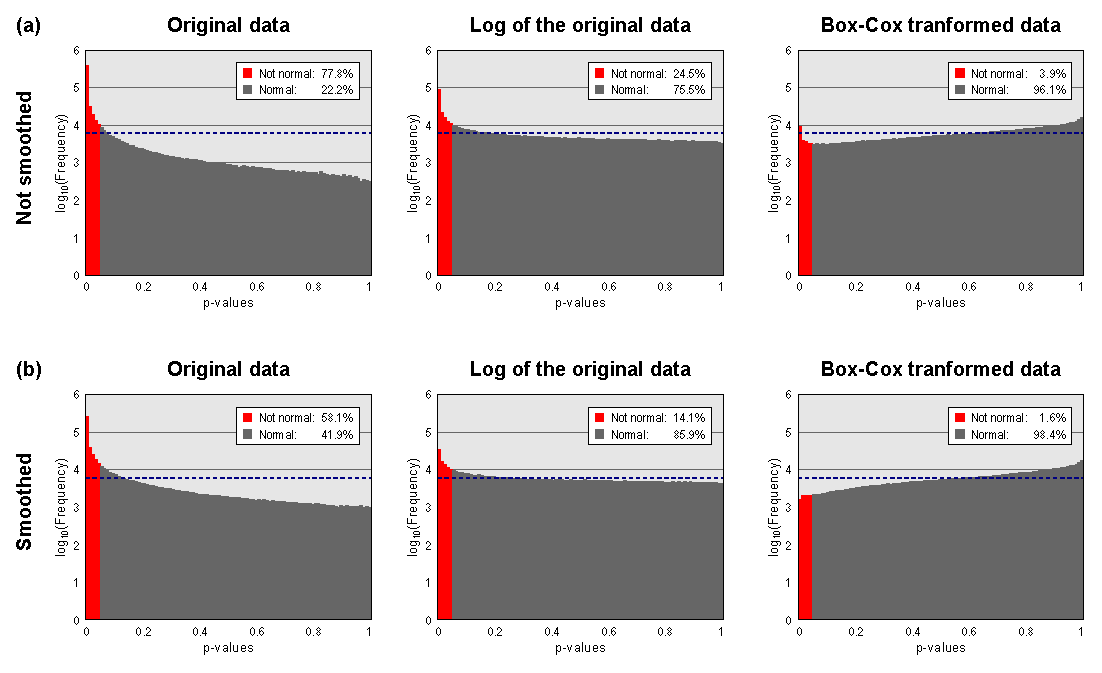
\includegraphics[width=14cm]{images/histograms.eps}
\caption[Results of the Shapiro--Wilk normality test.]{Distribution of the uncorrected p-values of the Shapiro--Wilk normality test. For normally distributed data, 5\% of these tests are always expected to be declared as not normal with a significance level of $\alpha=0.05$. Without transformation or smoothing, near 80\% are found as not normal. Logarithmic and Box--Cox transformations render the data more normally distributed. Observe that the frequencies are shown in logscale. The dashed line (\emph{blue}) is at the frequency that would be observed for uniformly distributed p-values.}
\label{fig:areal:histograms}
\end{figure}

\begin{figure}[!p]  % Figure Suppl 3
\centering
\includegraphics[width=14cm]{images/skewness.png}
\caption[Maps of the skewness of the areal data.]{Maps of the skewness of the areal data, before and after the Box--Cox transformation, and with and without smoothing. The distribution is positively skewed (lognormal) throughout most of the brain, and the transformation successfully brings the data to symmetry (normality). The histograms are shown in Figure \ref{fig:areal:skewness-hist}.}
\label{fig:areal:skewness}
\end{figure}

\begin{figure}[!p]  % Figure Suppl 4
\centering
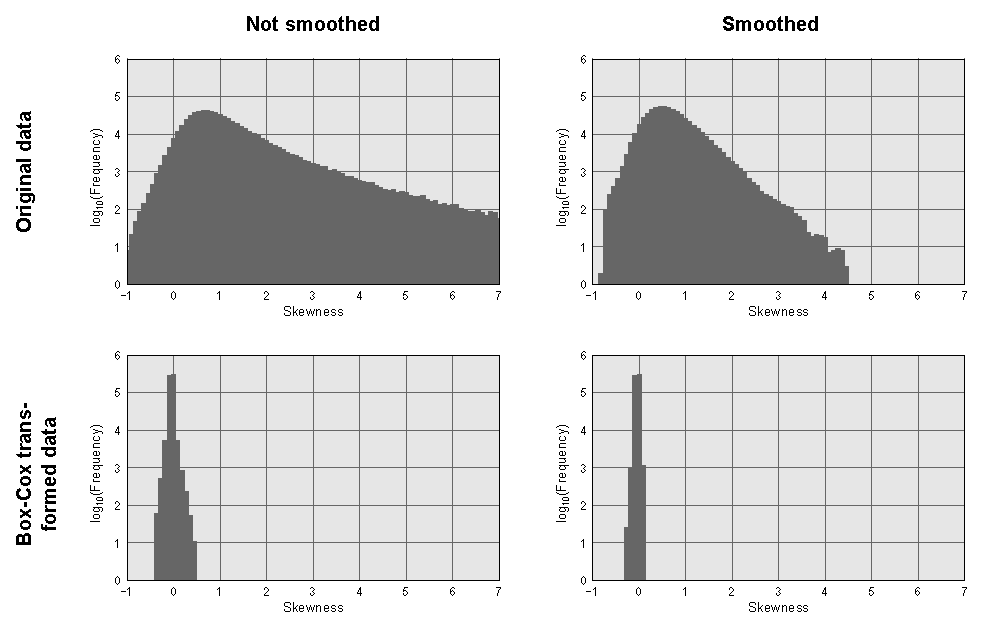
\includegraphics[width=14cm]{images/skewness-hist.eps}
\caption[Histograms of the skewness of the areal data.]{Histograms of the skewness of the areal data, before and after the Box--Cox transformation, and with and without smoothing. The distribution is positively skewed (lognormal) throughout most of the brain, and the transformation successfully brings the data to symmetry (normality). Note that the frequencies are shown in log scale. The corresponding maps are in Figure \ref{fig:areal:skewness}.}
\label{fig:areal:skewness-hist}
\end{figure}

\begin{figure}[!p]  % Figure Suppl 5
\centering
\includegraphics[width=14cm]{images/kurtosis.png}
\caption[Maps of the kurtosis of the areal data.]{Maps of the kurtosis of the areal data, before and after the Box--Cox transformation, and with and without smoothing. The distribution is leptokurtic throughout most of the brain, and the transformation renders the kurtosis closer to the same value as for the normal distribution, i.e.\ closer to the value 3. The histograms are shown in Figure \ref{fig:areal:kurtosis-hist}.}
\label{fig:areal:kurtosis}
\end{figure}

\begin{figure}[!p]  % Figure Suppl 6
\centering
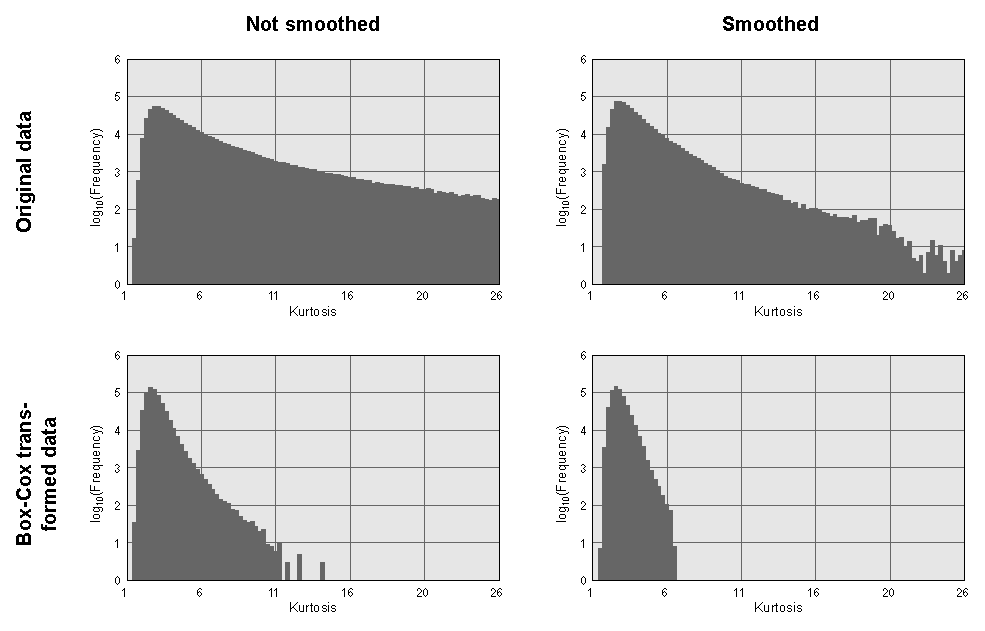
\includegraphics[width=14cm]{images/kurtosis-hist.eps}
\caption[Histograms of the kurtosis of the areal data.]{Histograms of the kurtosis of the areal data, before and after the Box--Cox transformation, and with and without smoothing. The distribution is leptokurtic throughout most of the brain, and the transformation renders the kurtosis closer to the same value as for the normal distribution, i.e.\ closer to the value 3.  Note that the frequencies are shown in log scale. The corresponding maps are in Figure \ref{fig:areal:kurtosis}.}
\label{fig:areal:kurtosis-hist}
\end{figure}

\begin{figure}[!p]  % Figure Suppl 2
\centering
\includegraphics[width=14cm]{images/boxcox.png}
\caption[Spatial distribution of the parameter $\lambda$.]{Distribution of the parameter $\lambda$ of the Box--Cox transformation across the brain: (\emph{a}) histogram and (\emph{b}) spatial map. When $\lambda$ approaches zero, the distribution of the underlying data is more lognormal.}
\label{fig:areal:boxcox}
\end{figure}

\subsection{Comparison with expansion/contraction methods}

A number of studies have analysed what has been called expansion or contraction of the cortical surface when compared to a reference brain. Different studies adopted different operational definitions for what these terms would be [e.g.\ compare \citet{Joyner2009}, \citet{Sun2009}, \citet{Hill2010}], and an unified approach has not been defined. Notwithstanding, the key difference between these methods and the proposed areal analysis is that, at the end of the processing pipeline, areal interpolation ensures the preservation of the amount (mass) of quantities, whereas these methods do not. Moreover, in the framework we present, a number of potential problems that may arise along the pipeline are explicitly addressed. These problems, along with the solutions we propose, are summarized in Table~\ref{tab:areal:compare}.

\begin{table}[!p]
\caption[Problems solved by the proposed method.]{The proposed framework for areal analyses addresses a number of potential problems that may arise along the processing pipeline.}
\begin{center}
{\small
\begin{tabular}{@{}m{42mm}<{\raggedright}m{44mm}<{\raggedright}m{43mm}<{\raggedright}@{}}
\toprule
Processing step &
Problem &
Solution \\
\midrule
Measurements assigned to vertices at the beginning of the analysis. &
Vertices do not hold or convey the same spatial information as the original faces. &
Analyze the faces directly. \\
\midrule
Registration methods that not necessarily produce smooth and invertible warps. &
Discontinuities on expansion or contraction that are not present in the actual brain. &
Use diffeomorphic registration methods. \\
\midrule
Interpolation based on points. &
Areal quantities are not preserved at any scale (local, regional or global). &
Use areal interpolation. \\
\midrule
Use of a standard brain to compute the same measurement that is later analysed. &
Results are interpretable only with respect to that same reference brain. &
Measure and analyse absolute quantities, not relative to some reference. \\
\midrule
Statistical analysis based on assumption of normality. &
The local surface area follows a lognormal distribution. &
Apply a data transformation. Use non-parametric methods. \\
\bottomrule
\end{tabular}}
\end{center}
\label{tab:areal:compare}
\end{table}

With a variety of expansion/contraction methods available, it is difficult to identify the best to which areal analysis could be compared. Here we retessellate the each subject brain in native space using the method described by \citet{Saad2004}. The expansion/contraction method was implemented using the following steps: (1) From the native surface geometry, perform the spherical transformation; (2) Perform the spherical registration to a standard brain; (3) Treat the coordinates $x$, $y$ and $z$ of the vertices from the native geometry as three independent scalar fields over the registed sphere, and interpolate these values to the common spherical grid using barycentric interpolation\footnote{The three scalar fields can also be treated as a single vector field and the barycentric interpolation can be performed in a single step as
\begin{displaymath}
\left[
\begin{array}{c}
x_{P} \\
y_{P} \\
z_{P}
\end{array} \right] = \left[
\begin{array}{ccc}
x_{A} & x_{B} & x_{C} \\
y_{A} & y_{B} & y_{C} \\
z_{A} & z_{B} & z_{C} \\
\end{array}
\right] \left[
\begin{array}{c}
\delta_{A} \\
\delta_{B} \\
\delta_{C}
\end{array} \right]
\end{displaymath} where $x,y,z$ represent the coordinates of the triangular face $ABC$ and of the interpolated point $P$, both in native geometry, and $\delta$ are the barycentric coordinates of $P$ with respect to the same face after the spherical transformation.}; (4) Use the interpolated coordinates, together with the same connectivity scheme between vertices as in the common grid, to construct a new model of the brain in a subject-specific geometry (Figure~\ref{fig:areal:retessellate}); (5) From this new model, compute the area per vertex and divide it by the area per vertex of the homologous point in the template. Call this measurement \emph{expansion/contraction}; (6) Optionally, smooth this quantity.

\begin{figure}[!tbp]  % Figure 7
\centering
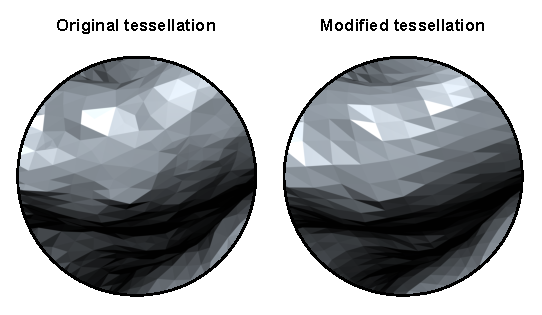
\includegraphics[width=10cm]{images/retessellate.eps}
\caption[Example of a retessellated surface.]{After barycentric interpolation of the coordinates in the surface of the sphere, a new, subject-specific retessellated model is constructed. Areas can be computed directly from the retessellated model and, once divided by the areas of the homologous vertices or faces of the reference brain, constitute the measurement of expansion/contraction.}
\label{fig:areal:retessellate}
\end{figure}

For comparison with the expansion/contraction method, the original facewise area was converted to vertexwise, therefore halving the spatial resolution of the areal data (see Section~\ref{sec:areal:conversion}). In this comparison, we addressed some of the problems presented in Table~\ref{tab:areal:compare}, namely, we registered using Spherical Demons, therefore ensuring smooth and invertible warps, and as target for registration, we used the study-specific template that produced the best results in Figure~\ref{fig:areal:registration}. Furthermore, the measurements were taken at the white surface, rather than the middle surface, as the last is more prone to be influenced by the cortical thickness. It is unclear if, when applicable, these aspects were taken care of in all the different studies that analysed some form of expansion/contraction.

After establishing an expansion/contraction procedure, there are still different ways to compare with areal analysis. The comparison can be made across subjects or across space, can be global or regional, and may or may not include smoothing. In Figure~\ref{fig:areal:expansion} we show that the average amount of area at each vertex did not produce a similar spatial map as the average expansion/contraction. Although the two methods follow remarkably different overall spatial patterns, when vertices across space were pooled together to produce a global measurement, they produced very similar results. Figure~\ref{fig:areal:scatter}a shows the relationship between the global cortical surface area, computed from the sum of the area at each vertex, and a global measure of expansion computed by averaging the expansion/contraction at each vertex across space.\footnote{Note that an exact measurement of expansion/contraction relative to the template can be produced simply by dividing the global area in native geometry by the area of the template geometry. In this case, the points in Figure~\ref{fig:areal:scatter}a would lie in a perfectly straight line, and nothing could be inferred about the relationship between regional variability on expansion estimates and global measurements.} The correlation was very high and helps to validate both methods as a whole. Likewise, when each vertex was analysed separately, the correlation across subjects was also very high, as shown in Figure~\ref{fig:areal:spatialfit}, with an $R^2$ above 0.9 throughout virtually the whole cortex. A spatial comparison of the average maps, on the other hand, showed a very poor relationship between both approaches, as shown in Figure~\ref{fig:areal:scatter}b. When looking at each individual subject, rather than at the average, the correlation across space was still relatively low, albeit not as poor: for the 168 hemispheres analysed, we found an average linear $R^2=0.572$, $\text{sd}=0.044$ without smoothing, and $R^2=0.491$, $\text{sd}=0.065$ after smoothing.

\begin{figure}[!tp]  % Figure 8
\centering
\includegraphics[width=14cm]{images/expansion.png}
\caption[Comparison with expansion/contraction methods (\textsc{i}).]{Average area (\emph{left panels}) or expansion/contraction (\emph{right panels}) per vertex, without (\emph{upper panels}) and with smoothing (\emph{lower panels}). Areal analyses and expansion/contraction differ across space. Smoothing has little global impact.}
\label{fig:areal:expansion}
\end{figure}

\begin{figure}[!tp]  % Figure 9
\centering
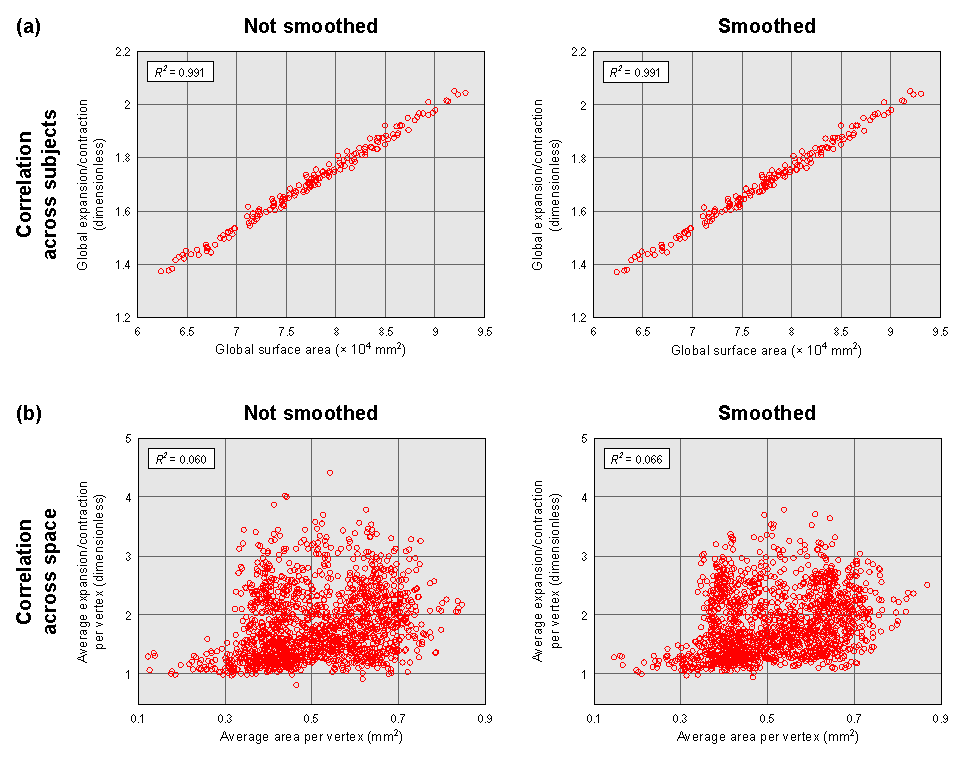
\includegraphics[width=14cm]{images/scatter.eps}
\caption[Comparison with expansion/contraction methods (\textsc{ii}).]{(\emph{a}) The sum of the area per vertex correlates well with the average across space of the expansion/contraction at each vertex (i.e. equivalent to a weighed sum considering each vertex as having the same initial area) for the 168 hemispheres analysed. For the expansion/contraction, this is not the same as computing the ratio between the global surface area in native geometry and of the template, in which case, the result would be a perfectly straight line. The high correlation implies that the regional differences in general compensate each other to produce a similar global effect. (\emph{b}) The correlation between average spatial maps across the 84 subjects, both hemispheres, is very poor between the methods. [Note that, for (\emph{b}), attempts to simultaneously plot all the $>$~300 thousand vertices would not produce meaningful plots in a small space; for this reason only 5\% of the vertices were randomly selected for plotting. The $R^2$ were computed from all vertices and, for both (a) and (b), the value corresponds to the goodness of a linear fit.]}
\label{fig:areal:scatter}
\end{figure}

\begin{figure}[!tp]  % Figure 10
\centering
\includegraphics[width=14cm]{images/spatialfit.png}
\caption[Comparison with expansion/contraction methods (\textsc{iii}).]{For each vertex, the linear relationship between areal analyses and expansion/contraction is very high across subjects, being above $R^2=$~0.90 virtually across the whole cortex.}
\label{fig:areal:spatialfit}
\end{figure}

These results suggest that, if each vertex is analysed in isolation, analysis of surface area and analysis of expansion/contraction tend to produce similar results. This is the case, for instance, using mass univariate \textsc{glm}-based approaches. However, for analysis that involve spatial information or that combine information across neighboring vertices, the results are expected to be rather dissimilar. The difference stems from the different units of measurement: areal analyses produce measurements in absolute units of area (e.g.\ mm$^2$), whereas expansion/contraction are relative to the a given reference. The result shown in Figure~\ref{fig:areal:spatialfit}, left panel, also demonstrate, indirectly, that areas measured in the retessellated brain with the resolution used correlate reasonably well with the areas obtained using areal interpolation, and so, have potential to be used as a fast approximation to areal interpolation (Section~\ref{sec:areal:implementation}). Conversely, expansion/contraction measurements can be obtained after areal interpolation simply by dividing the area per face (or per vertex) by its homologous in the reference brain.

\subsection{Validation and stability}

Measurements of surface area are valid as long as the surface reconstruction from \textsc{mr} images produces accurate representations of the cortex. The suggested reconstruction method has been previously validated \citep{Fischl2000}, and is widely used for cortical thickness measurements. Comparison between subjects at the face level depends on good matching of homologies and the registration method we suggest has, likewise, been previously validated \citep{Yeo2010, Klein2010}. As methods evolve, novel approaches for constructing surface representations of the cortex and for registration have potential to improve the overall quality of areal analyses. The validity of areal measurements other than surface area itself depend on each particular measurement technique.

To assess the stability across sessions and scanners, we compared \textsc{mr} images of the same subject acquired in three different sessions collected within a 1 year interval. The imaging protocol varied in terms of acquisition parameters, as well as the number of images used for averaging and improvements on signal and contrast-to-noise ratio. The details are summarized in Table~\ref{tab:areal:retest}. The estimated surface area produced by summing the facewise areas over the cortex after interpolation was very similar across tests, with the largest difference being 8.2\% between Tests \textsc{a} and \textsc{c} (see Table~\ref{tab:areal:retest}), with or without smoothing. The mean and standard deviation for facewise areas were virtually identical across tests, again regardless of smoothing. The pairwise Pearson correlation between the tests for the facewise data after registration and interpolation was above 0.80 without smoothing, and above 0.90 after smoothing with \textsc{fwhm} = 10~mm, showing that the procedure is robust at the face level, even under different scanning conditions and degrees of smoothing.

\begin{table}[!tp]
\caption[Stability of areal measurements.]{Stability and robustness of measurements after registration and interpolation were assessed using three test images of the same subject. The measurements were similar across tests, with similar variability across space and high spatial correlation.}
\begin{center}
{\footnotesize
\begin{tabular}{@{}l@{}m{33mm}<{\centering}@{}m{33mm}<{\centering}@{}m{33mm}<{\centering}@{}}
\toprule
{} & \textbf{Test A} & \textbf{Test B} & \textbf{Test C}\\
\midrule
Manufacturer and model & Siemens~\textsc{magnetom} Trio~3~T & Siemens~\textsc{magnetom} Trio/\textsc{tim}~3~T & Siemens~\textsc{magnetom} Allegra~3~T \\
Sequence & \textsc{mprage} & \textsc{mprage} & \textsc{mprage} \\
\textsc{te/ti/tr} (ms) & 3.04/785/2100 & 2.83/766/2200 & 2.74/900/2500 \\
Flip angle & 13$^{\circ}$ & 13$^{\circ}$ & 8$^{\circ}$ \\
Voxel size (mm) & $0.8 \times 0.8 \times 0.8$ & $0.8 \times 0.8 \times 0.8$ & $1.0 \times 1.0 \times 1.0$ \\
Number of acquisitions & 14 & 7 & 1 \\
Scan date & March 2008 & March 2008 & April 2009 \\
Cortical surface area (mm$^2$) & 176,996 & 177,098 & 180,949 \\
\midrule
\multicolumn{4}{l}{\textbf{Not smoothed}}\\
Average area per face (mm$^2$) & 0.2937 & 0.2939 & 0.3003 \\
Standard deviation             & 0.0938 & 0.0910 & 0.0962 \\
Correlation with Test A        &    --- & 0.8218 & 0.7589 \\
Correlation with Test B        & 0.8218 &    --- & 0.7863 \\
Correlation with Test C        & 0.7589 & 0.7863 &    --- \\
\midrule
\multicolumn{4}{l}{\textbf{Smoothed (\textsc{fwhm} = 10~mm)}}\\
Average area per face (mm$^2$) & 0.2935 & 0.2936 & 0.3000 \\
Standard deviation             & 0.0746 & 0.0712 & 0.0748 \\
Correlation with Test A        &    --- & 0.9509 & 0.9074 \\
Correlation with Test B        & 0.9509 &    --- & 0.9353 \\
Correlation with Test C        & 0.9047 & 0.9353 &    --- \\
\bottomrule
\end{tabular}}
\end{center}
\label{tab:areal:retest}
\end{table}

\section{Discussion}

\subsection{Registration}

To be valid, facewise analyses rely on the assumption that microscopic structures can be localized using as reference the features that are identifiable with \textsc{mri} and which drive the registration. Features with such localizing power are important because they help to ensure good overlap of homologous areas between subjects. Despite an implicit assumption already present in most imaging studies, only recently it has been demonstrated valid for some cytoarchitetonic areas when the references are the cortical folding patterns, even though for non-primary regions, the mismatch may still be substantial \citep{Fischl2008, Fischl2009, Hinds2008, Hinds2009, DaCosta2011}. Other features, some microscopic and detectable only under ultra-high field strengths \citep{Augustinack2005, Bridge2006, Duyn2007, Kim2009}, have the potential to be used as the reference as long as they are demonstrated to be markers of histologically or functionally defined areas, possibly replacing folding patterns altogether, or used to provide ancillary information. Myeloarchitectural features may be particularly useful for this application, for being resposible for most of the contrast observed with \textsc{mri} \citep{Geyer2011}. Likewise, areal analyses can be conducted after registration based on features derived from functional \textsc{mri} \citep{Sabuncu2010}.

Good matching of homologies, however, depends not only on the features used to guide the registration, but on the registration method itself. For facewise areal analyses, invertibility is necessary to prevent faces from being folded over others. In addition, methods that produce smooth warps are necessary to ensure that areal quantities are transferred smoothly, without abrupt variations. Such abrupt variations would only be acceptable if matching perfectly with areas where structure and/or function also changes abruptly. A spatial transformation that allows such perfect matching, however, cannot be obtained easily in practice, since these borders usually cannot be observed with current, conventional \textsc{mri} methods, and importantly, since many of the differences between regions are subtle and the transitions are gradual. However, invertibility and smoothness, as guaranteed by diffeomorphic methods, albeit important, may not suffice. Our results show that even methods that produce smooth varying warps can differ substantially with respect to how the areal quantities are shifted across the surface. It is possible that performance differences between these methods might be due to choices on regularization strategies and associated parameters \citep{Fischl1999_intersubject, Yeo2010}, instigating further reseach on selections that may produce the most accurate results \citep{Yeo2010b}. Our experiments also demonstrate that the choice of the target used for registration affects the distortion in areal measurements.

\subsection{Areal interpolation}

Areal interpolation allows direct analysis of areal quantities in absolute values, including the surface area itself. This is because it is the areal quantity proper that is conservatively transfered between grids. Therefore, there is no need to apply corrections due to stretches or shrinkages, such as using the Jacobian of the transformation \citep{Good2001}, nor due to the choice of the parametrizable surface \citep{Thompson1999}. Moreover, the results are interpretable directly with regard to the actual amount of tissue or other measurement under study, rather than relative to concepts as expansion/contraction, which are always relative to a given reference, and can create difficulties in interpretation and comparison across studies, either due to different definitions adopted by different authors, or due to the the need of a reference brain. Notwithstanding, after areal interpolation, it continues to be possible to divide the areas by the areas of the homologous faces or vertices of a reference brain, and so, obtain an expansion/contraction measurement. Moreover, areal quantities that are not area itself can also be divided by the area of each face or vertex in native geometry, thus converting these quantities to densities if necessary.

It should be emphasized that, as with other interpolation strategies, areal interpolation is not perfectly reversible, i.e.\ once the cortical area of a subject is transferred to a different grid, remapping back to the subject surface will not produce locally identical results, although the global areal quantity is always conserved. This is because within each face, the areal quantity is implicitly assumed to be homogeneously distributed. This only becomes a problem if low resolution meshes are used and if several back-and-forth iterations are performed.

\subsection{Statistical analysis of areal quantities}

There are a number of reasons that go beyond purely methodological considerations to justify the transformation of the data before statistical analysis. Measurements related to biological morphology, such as lengths, areas, volumes or weights, are well known to follow non-normal distributions. If the diameter of a structure, for instance, is normally distributed, inevitably both its cross section and its surface area follow skewed distributions, whereas its volume follows an even more skewed \citep{Kapteyn1916, Gaddum1945}. All these related measurements cannot be normally distributed simultaneously. The skewness is higher when the variability is relatively large in comparison to the measure of central tendency that best describes the data, such as the arithmetic or the geometric mean. If the non-normality is not considered, statistical models are likely to produce inaccurate results. In this scenario, a power transformation, such as the Box--Cox transformation, helps to identify subjacent, possibly causative, normally distributed effects.

The lognormal distribution, more specifically, is known to arise in a variety of biological processes. Of particular interest is the autocatalytic growth of tissue over time. The number of cells present on a tissue that grows in an unrestricted way can be given by the familiar formula $N=N_0e^{ct}$, where $N_0$ is the initial number of cells, and $t$ is the amount of time in which the cell grows under the circumstances represented by the constant $c$, a factor that incorporates a variety of influences, such as genetic and environmental. $N$ will be lognormally distributed if either $c$ or $t$ are normally distributed \citep{Koch1966, Limpert2001}. The finding that the facewise cortical surface area follows mostly lognormal distributions may suggest that the method may capture these biological effects. Such interpretation can only subsist under the tenets of accurate and smooth registration.

From a statistical perspective, permutation methods do not rely on normality, rendering them appropriate in a variety of situations in which this assumption is not tenable. Nevertheless, the data should, still, undergo a transformation. As discussed above, the reason is not merely to conform to normality, although that comes as a bonus, but also to ensure that underlying biological effects, either multiplicative or proportionally dependent upon an initial value, can be treated as additive in a linear model \citep{Christensen2002}. Areal quantities that are not the cortical surface area itself can, notwithstanding, be distributed differently, and the framework for statistical analysis outlined in the Methods section appears generic enough to accomodate a variety cases. The Box--Cox transformation has yet another advantage when used in combination with permutation methods under multiple testing conditions: the more stable variance after the transformation allows the distribution of the statistic under null hypothesis to become more similar across tests, allowing \textsc{fwer} to be controlled at a level closer to its nominal value using the distribution of the maximum statistic.

\subsection{Box--Cox and log-normality}

An interesting aspect related to the Box--Cox transformation is that here it was used as a metric to quantify how normal or log-normal the data are. This has clear applications in biology. Tissue growth that depends on cellular multiplication is exponential, with a constant factor that is often normally distributed, resulting in tissue size that is log-normally distributed \citep[for a discussion, see][]{McAlister1879, Koch1966, Koch1969}. Measurements of the final tissue size in different individuals, however, does not perfectly conform to the log-normal due to external influences that may hinder tissue growth. Moreover, it is not always possible to measure the final amount of tissue that is the product of a single lineage of self-multiplicative cells. The combination of different cell lineages, each with their own growth rate, as well as external influences, tend to produce a distribution that is more normally (Gaussian) distributed. This appears to be the case of the cerebral cortex, with a \emph{distribution gradient} between these two extremes of normality and log-normality. Estimating the parameter $\lambda$ allows one to estimate also how closer to normal or log-normal certain measurements are. If $\lambda \approx 0$, the original data tend to be log-normally distributed, whereas if $\lambda \approx +1$, the data can be considered approximately more normally distributed.

\subsection{Further developments and potential applications}

Facewise analyses offer the possibility of studying surface area at a much finer scale than previously. This is a feature of interest in many research fields across the neurosciences, as well as in medicine. Although the same applies to vertexwise cortical thickness, thickness and area provide different and complementary insights into processes underlying the development of the brain and disorders \citep{Voets2008, Winkler2010, SanabriaDiaz2010}.

Provided that the neurons in the cortex retain largely their same relative positions as the progenitor cells in the embryo \citep{Rakic1988, Rakic2009a, Pierani2009, Clowry2010}, facewise comparison of surface area allows one to hypothesize about ontogenetic processes to the extent that they can be observed and localized with \textsc{mri}, even long after the end of phases of massive tangential cellular proliferation. Until now, this kind of study could not be performed, either due to lack of methods to analyse cortical surface area without the constrains imposed by regions of interest, or due to inherent limitations of methods based on expansion or contraction.

The study of local cortical surface area offers, moreover, new possibilities for connectivity analyses, as the need for parcellations based on macroscopic anatomy is obviated. Indeed, the results of connectivity analyses are known to be influenced by the choice of the parcellation that define nodes of putative neuronal networks \citep{Butts2009, Rubinov2010}. Notwithstanding, if a given set of regions is derived from a different method \citep{Beckmann2009a, Nelson2010}, these can be directly associated with their corresponding surface-based areas or areal quantities by means of areal interpolation.

Another potential application is for genetic analyses. Given that cortical surface area and thickness are both heritable, yet genetically not correlated \citep{Panizzon2009, Winkler2010}, these traits, separately, can be used in a framework similar to voxelwise genome-wide association studies (v\textsc{gwas}) \citep{Stein2010}. Identification of genes that influence surface area have potential to elucidate a myriad of developmental, neurologic and psychiatric disorders.

\section{Chapter conclusion}

We presented an interpolation method for between-subject analyses of cortical surface area. The method is also suitable for other quantities that are areal by nature and which require mass conservation (pycnophylactic property) during interpolation and analysis. We demonstrated that, when the quantity under study is surface area itself, the distribution of the data does not follow a normal distribution, being instead better characterized as lognormal, and proposed a framework for statistical analysis and inference.
\cleardoublepage \include{40permutation}
\cleardoublepage \chapter{Combination inference}
\label{sec:comb:combination}
\setstretch{\lspac}

\section{Introduction}

% IUT
% Conjunction/disjunction
% partial, marginal
% F-tests, rejection regions
% FWER 
% Meta-analysis
% Diagram, comparison
% Relationship with cognition, biological interpretation

% Implementation aspects: avoid being close to 1, etc
% Common framework for different tests

% Uses of NPC
% - Different modalities
% - Same modality, different aspects -- ICs, DTI scalars, thick/area
% - Repeated measurements
% - Non-orthogonal studies

% Philosophical questions: should we combine or dissect?

The previous chapter discussed how permutation methods, for being free of various assumptions related to classical parametric tests, could better adapt to the growing variety of experimental imaging methods. In this chapter, these ideas are further extended to non-parametrically allow \emph{joint inference} on more than one modality, that is, how to infer about hypotheses concerning these modalities when more than one image is available for each subject. Examples of such modalities include the same cited in Chapter~\ref{sec:comb:permglm}, such as, but not limited to, positron emission tomography (\textsc{pet}), functional magnetic resonance imaging (\textsc{fmri}), tensor-based morphometry (\textsc{tbm}), diffusion tensor imaging (\textsc{dti}), cortical thickness and surface area, cerebral perfusion, as well as various others.

Further to these examples, it is also the case that the same imaging modality is often subdivided so as to better characterise certain physical properties --- including morphology and function --- of the biological tissue. As an example, diffusion-weighted images are often used to generate maps of fractional anisotropy (\textsc{fa}), mean diffusivity (\textsc{md}), radial diffusivity (\textsc{rd}), as well as lengths of the eigenvectors of the diffusion tensor and other measurements. Another example is the use of independent component analysis (\textsc{ica}) to decompose \textsc{fmri} time series into a set of timecourses and spatial maps. Only some of these components might be of actual interest, or the effect of interest might be split into more than one; in either case, a strategy that could combine the information from these into a single inferential step tends to be more meaningful than various separate tests.

Historically, as in the case of the permutation tests discussed in Chapter~\ref{sec:comb:permglm}, Ronald A.\ Fisher was among the first to propose such joint analysis of various tests. In the fourth edition of his now classical book \textit{Statistical Methods for Research Workers} \citep{Fisher1932}, his approach was described rather succinctly:

\begin{quote}
\emph{When a number of quite independent tests of significance have been made, it sometimes happens that although few or none can be claimed individually as significant, yet the aggregate gives an impression that the probabilities are on the whole lower than would often have been obtained by chance. It is sometimes desired, taking account only of these probabilities, and not of the detailed composition of the data from which they are derived, which may be of very different kinds, to obtain a single test of the significance of the aggregate, based on the product of the probabilities individually observed.}

\emph{The circumstance that the sum of a number of values of $\chi^{2}$ is itself distributed in the $\chi^{2}$ distribution with the appropriate number of degrees of freedom, may be made the basis of such a test. For in the particular case when $n=2$, the natural logarithm of the probability is equal to $\frac{1}{2}\chi^{2}$. If therefore we take the natural logarithm of a probability, change its sign and double it, we have the equivalent value of $\chi^{2}$ for 2 degrees of freedom. Any number of such values may be added together, to give a composite test, using the Table of $\chi^{2}$ to examine the significance of the result. \hfill --- \citet{Fisher1932}}
\end{quote}

The logic of this test is based on the fact that the probability of rejecting the global null hypothesis is related to intersection of the probabilities of each individual test, i.e., $\prod_{i} P_{i}$. However, $\prod_{i} P_{i}$ is not uniformly distributed, even if the null is true for all partial tests, and cannot be used itself as the joint significance level for the global test. To remediate this fact, some interesting properties and relationships among distributions of random variables were exploited by Fisher and embodied in the succinct excerpt above:

\paragraph{The logarithm of uniform is exponential} The cumulative distribution function (cdf) of an exponential distribution is $F(x)=1- e^{-\lambda x}$ where $\lambda$ is the rate parameter, the only parameter of this distribution. The inverse cdf is, therefore, given by $x = -\dfrac{1}{\lambda}\ln(1-F(x))$. $F(x)=P$ is a random variable uniformly distributed in the interval $[0, 1]$, and so is $1-P$, and it is immaterial to differ between them. As a consequence, the same can be written as $x = -\dfrac{1}{\lambda}\ln(P)$, where $P \sim \mathcal{U}(0,1)$, which highlights the fact that the negative of the natural logarithm of a random variable distributed uniformly between 0 and 1 follows an exponential distribution with rate parameter $\lambda=1$.

\paragraph{An exponential with rate 1/2 is $\chi^2$ distributed} The cdf of a chi-squared distribution with $\nu$ degrees of freedom, i.e. $\chi^{2}_{\nu}$, is given by $F(x; \nu) = \dfrac{\int_{0}^{x/2} t^{\frac{\nu}{2}-1}e^{-t}{\rm d}t}{\left(\frac{\nu}{2}-1\right)!}$. If $\nu=2$, the expression simplifies to $F(x; \nu=2) = 1-e^{-x/2}$. In other words, a $\chi^{2}$ distribution with $\nu=2$ is equivalent to an exponential distribution with rate parameter $\lambda=1/2$.

\paragraph{The sum of chi-squared is also chi-squared} The moment-generating function (mgf) of a sum of independent variables is the product of the mgfs of the respective variables. The mgf of a $\chi^{2}_{\nu}$ is $M(t) = (1-2t)^{-\nu/2}$. The mgf of the sum of $K$ independent variables that follow each a $\chi^{2}_{2}$ distribution is then given by $M_{\text{sum}}(t) = \prod_{i=1}^{K} (1-2t)^{-2/2} = (1-2t)^{-K}$, which also defines a $\chi^{2}$ distribution, however with degrees of freedom $\nu=2K$.

With these facts in mind, the product $\prod_{i} P_{i}$ can be transformed into a p-value that is uniformly distributed when the global null is true. The product can be converted into a sum by taking the logarithm. And as shown above, the logarithm of uniformly distributed variables follows an exponential distribution with rate parameter $\lambda=1$. Multiplication of each $\ln(P_{i})$ by 2 changes the rate parameter to $\lambda=1/2$ and makes this distribution equivalent to a $\chi^{2}$ distribution with degrees of freedom $\nu=2$. The sum of $k$ of these logarithms also follow a $\chi^2$ distribution, now with $\nu=2K$ degrees of freedom, i.e., $\chi^{2}_{2K}$. Thus, the statistic for the Fisher method is given by $T_{\text{Fisher}}$ $=$ $-2 \sum_{i=1}^{K} \ln(P_{i})$, with $T_{\text{Fisher}}$ following a $\chi^{2}_{2K}$ distribution, from which a p-value for the global hypothesis can be easily obtained.

The elegance of the combination strategy devised by Fisher resides in that it depends solely on the uniformity of the distribution of the p-values for each of the separate $K$ tests under the null hypothesis, something that, by definition, is always attained whenever a statistical test is exact. This also renders the test, in a certain sense, non-parametric, although arguably, the number of tests can be considered a parameter upon which the resulting combined statistic depends.

\section{Parametric combination strategies}

The logic followed by Fisher is helpful to understand the behaviour of various other approaches. All of them pool a summary statistic from the original tests to produce a new, joint statistic. This joint statistic is used to assess significance of the aggregate of the tests. Consider $K$ independent tests, each with their respective p-values $p_{k}$, $k=\{1$, $\ldots$, $K\}$. These tests can also be called \emph{partial tests} \citep{Pesarin2010}, and each can, individually, be declared significant or not at certain level $\alpha$. For each combining method, an overall statistic $T_{\text{(method)}}$ is obtained, from which a p-value, $P_{\text{(method)}}$, is computed to reject or not, at a given significance level $\gamma$, the \emph{global null hypothesis}\footnote{Also called \emph{conjunction of null hypotheses} \citep{Benjamini2008}.} that there is no effect for all partial tests. Here the same significance level $\alpha$ is used for all of the partial tests, although some methods permit the use of a different $\alpha$ for each.

A list of these methods is presented below, in chronological order as they were published, and summarised in Table~\ref{tab:comparisonC}. All of these could be termed as ``non-parametric'' for not depending on the underlying distribution of the data for the original tests, only on their p-values, although most are still ``parametric'' in the sense that most have a known asymptotic distribution for their respective statistic $T_{\text{(method)}}$ if certain assumptions are met for each case. As a general rule, the parametric p-values of all these methods are supposed to be exact if the tests are independent, whereas some are robust to a certain degree of non-independence, even if independence was assumed during their derivation.

\begin{table}[b!]
\caption[Summary of different combining functions.]{\emph{(Page \pageref{tab:comparisonT})} Several methods are available to combine inference from multiple tests. In the table, $T$ is the statistic for each corresponding method and $P$ its significance, i.e.\ the probability by chance of a statistic as extreme as $T$ or higher for each method.
The respective null hypothesis (global null or conjunction null) is rejected if $P \leqslant \gamma$.
All methods are shown as function of the partial p-values, $p_{k}$. However, for certain methods, the test statistic from the partial tests, if available, can be used directly (e.g. Stouffer, Winer).
$K$ is the number of tests being combined,
$p_{k}$, $k=\left\{1,2,\ldots,K\right\}$ are the partial p-values,
$w_{k}$ are positive weights assigned to the respective $p_{k}$,
$p_{(r)}$ are the $p_{k}$ with rank $r$ in ascending order (most significant first),
$\alpha$ is the significance level for the partial tests,
$u$ is the minimum number of tests where the null should be rejected for a partial conjunction null test,
$I(\cdot)$ is an indicator function that evaluates as 1 if the condition is satisfied, 0 otherwise,
$\lfloor \cdot \rfloor$ represents the floor function,
$\chi^{2}_{\nu}$ is the cumulative distribution function (cdf) for a $\chi^{2}$ distribution, with the $\nu$ degrees of freedom,
$t_{\text{cdf}}$ is the cdf of the Student's $t$ distribution with degrees of freedom $\nu$, and $t_{\text{cdf}}^{-1}$ its inverse,
$\Phi$ is the cdf of the normal distribution with mean $\mu$ and variance $\sigma^{2}$, and $\Phi^{-1}$ its inverse,
$F$ and $G$ are the cdf of arbitrary, yet well chosen, distributions.
For details and references, consult the main text.}
\label{tab:comparisonC}
\end{table}

\begin{sidewaystable}
\begin{center}
{\footnotesize
\begin{tabular}{@{}m{3.6cm}@{}m{6.7cm}<{\raggedright}@{}m{12.2cm}<{\raggedright}@{}}
\toprule
\label{tab:comparisonT} Method & Test statistic ($T$) & Significance ($P$)\\
\midrule
Tippett &
$\min_{k} \left(p_{k}\right)$ &
$1-\left(1-T\right)^{K}$ \\
\midrule[0pt]
Fisher &
$-2 \sum_{k=1}^{K} \ln\left(p_{k}\right)$ &
$1-\chi^{2}\left(T;\;\nu=2K\right)$\\
\midrule[0pt]
Pearson--David &
$-2\min\left(\sum_{k=1}^{K} \ln\left(p_{k}\right),\sum_{k=1}^{K} \ln\left(1-p_{k}\right)\right)$ &
$1-\chi^{2}\left(T;\;\nu=2K\right)$\\
\midrule[0pt]
Stouffer &
$\frac{1}{\sqrt{K}} \sum_{k=1}^{K} \Phi^{-1}\left(1-p_{k}\right)$ &
$1-\Phi\left(T;\;\mu=0,\;\sigma^2=1\right)$\\
\midrule[0pt]
Wilkinson &
$\sum_{k=1}^{K} I\left(p_{k}\leqslant\alpha\right)$ &
$\sum_{k=T}^{K}\binom{K}{k}\alpha^{k}(1-\alpha)^{K-k}$ \\
\midrule[0pt]
Good &
$\prod_{k=1}^{K} p_{k}^{w_{k}}$ &
$\sum_{k=1}^{K}w_{k}^{K-1}T^{1/w_{k}}\left(\prod_{i=1}^{k-1}\left(w_{k}-w_{i}\right)^{-1}\right) \left(\prod_{i=k+1}^{K}\left(w_{k}-w_{i}\right)^{-1}\right)$\\
\midrule[0pt]
Lancaster &
$\sum_{k=1}^{K} w_{k}F_{k}^{-1}\left(1-p_{k}\right)$ &
$1-G\left(T\right)$\\
\midrule[0pt]
Winer &
$\sum_{k=1}^{K}t_{\text{cdf}}^{-1}\left(1-p_{k};\;\nu_{k}\right)\left/\sqrt{\sum_{k=1}^{K}\frac{\nu_{k}}{\nu_{k}-2}}\right.$ &
$1-\Phi\left(T;\;\mu=0,\;\sigma^2=1\right)$\\
\midrule[0pt]
Edgington &
$\sum_{k=1}^{K} p_{k}$& 
$\sum_{j=0}^{\lfloor T \rfloor}(-1)^j \binom{K}{j}\frac{\left(T-j\right)^K}{K!}$ \\
\midrule[0pt]
Mudholkar--George &
$\frac{1}{\pi}\sqrt{\frac{3(5K+4)}{K(5K+2)}}\sum_{k=1}^{K} \ln\left(\frac{1-p_{k}}{p_{k}}\right)$ &
$1-t_{\text{cdf}}(T;\;\nu=5K+4)$\\
\midrule[0pt]
Friston &
$\max_{k} \left(p_{k}\right)$ &
$T^{K}$ (global null) or $T^{K-u+1}$ (partial conjunction null)\\
\midrule[0pt]
Darlington--Hayes &
$\frac{1}{r} \sum_{k=1}^{r} \Phi^{-1}\left(1-p_{(k)}\right)$ &
Computed through Monte Carlo methods. Tables are available.\\
\midrule[0pt]
Zaykin &
$\prod_{k=1}^{K} p_{k}^{I\left(p_{k} \leqslant \alpha\right)}$ &
$\sum_{k=1}^{K}\binom{K}{k}\left(1-\alpha\right)^{K-k}\left(I\left(T> \alpha^{k}\right) \alpha^{k}  + I\left(T\leqslant \alpha^{k}\right)T\sum_{j=0}^{k-1}\frac{\left(k\ln \alpha - \ln T\right)^{j}}{j!}\right)$\\
\midrule[0pt]
Dudbridge--Koeleman &
$\prod_{k=1}^{r} p_{(k)}$ &
$\binom{K}{r+1}\left(r+1\right) \int_0^1\left(1-t\right)^{K-r-1}\left(I\left(T> t^{r}\right) t^{r} +I\left(T \leqslant t^{r}\right) T \sum_{j=0}^{r-1}\frac{\left(r\ln t - \ln T\right)^{j}}{j!}\right)\mathrm{d}t$ \\
\midrule[0pt]
Nichols &
$\max_{k} \left(p_{k}\right)$ &
$T$ (conjunction null)\\
\midrule[0pt]
Taylor--Tibshirani &
$\frac{1}{K} \sum_{k=1}^{K} \left(1-p_{(k)}\frac{K+1}{k}\right)$ &
$1-\Phi\left(T;\;\mu=0,\;\sigma^2 \approx \frac{1}{K}\right)$ \\
\midrule[0pt]
Jiang &
$\frac{1}{K} \sum_{k=1}^{K} I\left(p_{(k)}\leqslant \alpha \right)\left(1-p_{(k)}\frac{K+1}{k}\right)$ &
Computed through Monte Carlo methods.\\
\bottomrule
\multicolumn{3}{l}{\emph{See caption on page \pageref{tab:comparisonC}.}}
\end{tabular}}
\end{center}
\end{sidewaystable}

\paragraph{Tippett} This is the oldest and probably the simplest of the combination methods, having appeared in \citet{Tippett1931}. The combined test statistic is simply the minimum p-value across all partial tests, i.e. $T_{\text{Tippett}} =$ $\min_{k} \left(p_{k}\right)$. The probability is computed as $P_{\text{Tippett}} = 1-\left(1-T_{\text{Tippett}}\right)^{K}$.

\paragraph{Fisher} This is certainly the most well known of the combination strategies. It appeared in \citet{Fisher1932} and follows from the idea of treating the joint probability as the intersection of all partial tests, which is given by their product $\prod_{k} p_{k}$. A statistic for the global hypothesis can be constructed as $T_{\text{Fisher}} =$ $-2 \sum_{k} \ln\left(p_{k}\right)$, as shown earlier in this chapter, which follows a $\chi^2$ distribution with $2k$ degrees of freedom, and from which an uniformly distributed significance level, $P_{\text{Fisher}}$, can be obtained.

\paragraph{Pearson--David} The same product suggested by Fisher, $\prod_{k} p_{k}$, was used by \citet{Pearson1933} to test equality of distributions. \citet{David1934} discussed that a similar test could be used with $\prod_{k} (1-p_{k})$ and suggested using the most extreme of these two products as the statistic, a view later shared by Pearson himself \citep{Pearson1934}. The test statistic is, therefore, given by $T_{\text{Pearson--David}}=$ $-2\min\big(\sum_{k} \ln\left(p_{k}\right),$ $\sum_{k} \ln\left(1-p_{k}\right)\big)$, which, as in the Fisher method, follows a $\chi^{2}$ distribution with $2k$ degrees of freedom, and from which the significance $P_{\text{Pearson--David}}$ can be computed.\footnote{Historical details regarding this method are recounted in \citet{Owen2009}. The authors also comment that the significance level could be doubled to account for the fact that two tests are being performed, although this is not in the original publications.}

\paragraph{Stouffer} This method appeared as a footnote in the report of the sociological study conducted among veterans of the World War \textsc{ii} by \citet{Stouffer1949}. The idea is to convert the p-values to normally-distributed $z$-scores, sum these scores, and compute a new p-value. The conversion to a normal distribution is irrespective to the distributions from which the partial p-values, $p_{k}$, may have arisen. The test statistic is given by $T_{\text{Stouffer}} =$ $\frac{1}{\sqrt{K}} \sum_{k} \Phi^{-1}\left(1-p_{k}\right)$, where $\Phi^{-1}$ is the inverse cumulative distribution function (cdf) of the normal distribution (i.e.\ the probit function). The statistic $T_{\text{Stouffer}}$ follows a normal distribution with zero mean and unit variance, from which a probability $P_{\text{Stouffer}}$ can be obtained.

\paragraph{Wilkinson} The probability of observing $r$ significant p-values at level $\alpha$ out of the $K$ tests performed can be computed using a binomial expansion as proposed by \citet{Wilkinson1951}. The statistic $T_{\text{Wilkinson}}$ is simply $r$, and the probabilty of finding no more or less than $r$ by chance is given by $P_{\text{Wilkinson}} =$ $\sum_{k=r}^{K}\binom{K}{k}\alpha^{k}(1-\alpha)^{K-k}$. If the partial p-values are sorted in ascending order, $p_{(1)} \leqslant p_{(2)} \leqslant \ldots \leqslant, p_{(K)}$, and if the significance level is defined as $\alpha=p_{(1)}$, the approach is equivalent to the Tippett method. Note that the probability does not depend on the actual probabilities for the partial tests, but only on $r$ and $\alpha$.

\paragraph{Good}  A generalisation of the Fisher method, and which assigns arbitrary, unequal positive weights $w_{k}$ for each of the p-values of the partial tests, was suggested by \citet{Good1955}. Each partial test can be weighted according to some criteria, for instance, the sample size for each of the partial test, the number of degrees of freedom, or some other desirable feature, such as ecological or internal validity \citep{Rosenthal1978}. The statistic is given by $T_{\text{Good}}=\prod_{k}p_{k}^{w_{k}}$, and its significance can be assessed as $P_{\text{Good}}=$ $\sum_{k}W_{k}T_{\text{Good}}^{1/w_{k}}$, where $W_{k}=$ $w_{k}^{K-1}$ $\left(\prod_{i=1}^{k-1}\left(w_{k}-w_{i}\right)^{-1}\right)$ $\left(\prod_{i=k+1}^{K}\left(w_{k}-w_{i}\right)^{-1}\right)$.

\paragraph{Lipt\'{a}k} Another generalised combined statistic can be produced using the inverse cdf, $F^{-1}$, of the $p_{k}$, summing the values of the statistics, and computing a new p-value for the global null using the cdf $G$ of the sum of the statistics, a method proposed by \citet{Liptak1958}. Each summand can be arbitrarily weighted, as in the Good method. In principle, any continuously increasing function with support in the interval $[0;\; 1]$ can be used for $F$, albeit a more obvious choice is the cdf of the normal distribution, which can be used as both $F$ and $G$, and which makes the approach virtually identical to the Stouffer method if all weights are 1 \citep{vanZwet1967}. In this case, the statistic for the method is given by $T_{\text{Lipt\'{a}k}} =$ $\sum_{k} w_{k}\Phi^{-1}\left(1-p_{k}\right)$, which follows a normal distribution with zero mean and variance $K$. $F$ can also be a $\chi^{2}_{\nu}$ distribution, in which case, and also when all $w_{k}=1$, $G$ is a $\chi^{2}_{K\nu}$ distribution. If $\nu=2$, the approach is equivalent to the Fisher method.

\paragraph{Lancaster} While Lipt\'{a}k method generalises combining strategies such as Fisher and Stouffer, the Lancaster method \citep{Lancaster1961} further generalises the Lipt\'{a}k approach by allowing different $F^{-1}_{k}$ for each partial test. Choices for $F^{-1}_{k}$ include, for instance, the cdf of the gamma distribution with scale parameter $\theta=2$, possibly with different shape parameters taking the place of the weights $w_{k}$ for each partial test. If the weights are all positive integers, the significances can be assessed from the cdf of a $\chi^{2}$ distribution, with degrees of freedom $\nu=2\sum_{k}w_{k}$ \citep{Berk1979}.

\paragraph{Winer} A combination strategy that resembles the Stouffer method, but uses Student's $t$ statistics, rather than $z$-scores was proposed by \citet{Winer1962}. The idea is to sum the $t$ statistics for all the $K$ partial tests, and normalising the sum so that the resulting statistic follows a standard normal distribution. The normalisation is based on the fact that the variance of the $t$ distribution can be determined from its the degrees of freedom $\nu$ as $\nu/(\nu-2)$. The statistic for this method is given by $T_{\text{Winer}}=$ $\sum_{k}t_{k}\left/\sqrt{\sum_{k}\frac{\nu_{k}}{\nu_{k}-2}}\right.$. The Winer method cannot be applied if $\nu_{k} \leqslant 2$ for any of the partial tests. Moreover, $\nu_{k}$ should not be too small for the normal approximation to be reasonably valid (e.g., $\nu_{k} \geqslant 10$). The Winer method is a particular case of the Lancaster method. {\color{orange} \emph{this all needs checking with the book!}}

\paragraph{Edgington} The probability of observing, due to chance, a value equal or smaller than the sum of the partial p-values, $T_{\text{Edgington}}=\sum_{k} p_{k}$, was proposed by \citet{Edgington1972} as a more powerful alternative to the Fisher method. This probability can be calculated as $P_{\text{Edgington}} =$ $\frac{T^K}{K!}$ when $T \leqslant 1$, where $T$ is the $T_{\text{Edgington}}$ statistic. More generally, or if $T>1$ the probability can be computed as $P_{\text{Edgington}} =$ $\sum_{j=0}^{\lfloor T \rfloor}(-1)^j \binom{K}{j}\frac{(T-j)^K}{K!}$, where $\lfloor \cdot \rfloor$ is the floor function.

\paragraph{Mudholkar--George} It is possible to use a simple logit transformation to compute a statistic that approximates a scaled version of the Student's $t$ distribution, as shown by \citet{Mudholkar1979}. The scaling can be applied to the result of the logit transformation itself, such that the statistic is computed as $T_{\text{Mudholkar--George}}$ $=$ $\frac{1}{\pi}\sqrt{\frac{3(5K+4)}{K(5K+2)}}\sum_{k} \ln\left(\frac{1-p_{k}}{p_{k}}\right)$, which follows a $t$ distribution with $5K+4$ degrees of freedom.

\paragraph{Friston (global null)} \citet{Friston1999} proposed the use of the minimum statistic, or equivalently, the maximum $p_{k}$, across the $K$ tests as a way to test the null hypothesis of no effect for all the tests. The fact that it had originally been called a ``conjunction'' caused some confusion in the literature, because the eventual rejection of the global null cannot be used to infer that the null for each of the partial tests are all rejected, as it would be in a logical conjunction \citep{Nichols2005}. The statistic for this method can be expressed in terms of the p-values for the partial tests as $T_{\text{Friston}}=$ $\max_{k} \left(p_{k}\right)$, and its significance can be assessed as $P_{\text{Friston-GN}}=T^{K}_{\text{Friston}}$. The Friston method is equivalent to the Wilkinson method if $\alpha=p_{(K)}$ and so, $r=K$.

\paragraph{Darlington--Hayes} In a discussion about pooling p-values for meta-analysis, \citet{Darlington2000} raised a number of limitations of these methods, and proposed a modification over the Stouffer method that would address some of these concerns. The modified method, called \emph{Stouffer-max}, uses as test statistic the mean of the $r$ highest $z$-scores, i.e. $T_{\text{Darlington--Hayes}} =$ $\frac{1}{r} \sum_{k=1}^{r} \Phi^{-1}\left(1-p_{(k)}\right)$, rather than the normalised sum all the $z$-scores as in the Stouffer method. When $r=1$, it is equivalent to the Tippett method, whereas when $r=K$, equivalent to the original Stouffer. Significances can be computed for intermediate values of $r$ through Monte Carlo simulation, and the authors provided tables with critical values.

\paragraph{Zaykin} This method, called \emph{truncated product method} (\textsc{tpm}) was proposed by \citet{Zaykin2002} as a way to combine features of the Fisher and Wilkinson methods. The statistic is given by $T_{\text{Zaykin}}=$ $\prod_{k=1}^{K} p_{k}^{I\left(p_{k} \leqslant \alpha\right)}$, where $I\left(\cdot\right)$ is an indicator function that evaluates as 1 if the given condition is satisfied, and 0 otherwise. In other words, the statistic is the product of only the partial p-values that are significant at the level $\alpha$, whereas in the Fisher method, all p-values are used. The significance for the combination is given by $P_{\text{Zaykin}} =$ $\sum_{k=1}^{K}\binom{K}{k}\left(1-\alpha\right)^{K-k}$ $\Big(I\left(T > \alpha^{k}\right) \alpha^{k}$ $+$ $I\left(T \leqslant \alpha^{k}\right)T\sum_{j=0}^{k-1}\frac{\left(k\ln \alpha - \ln T\right)^{j}}{j!}\Big)$, where $T$ is $T_{\text{Zaykin}}$.  If $\alpha = \min_{k}\left(p_{k}\right)$, then the approach is equivalent to the Tippett method. If $\max_{k}\left(p_{k}\right) \leqslant \alpha \leqslant 1$, the approach is equivalent to the Fisher method. Although exact, computationally the expression for $P_{\text{Zaykin}}$ is prone to over/underflows for certain combinations of large $K$ and $\alpha$, and because of this, when a global significance cannot be obtained analytically, Monte Carlo methods can be used.

\paragraph{Dudbridge--Koeleman} While the Zaykin method combines only the partial tests that are significant at the level $\alpha$, it is also possible to create a statistic that combines only the most $r$ significant tests, where $r$ is specified in advance. This method was proposed by \citet{Dudbridge2003} and called \emph{rank truncated product} (\textsc{rtp}). The main benefit of this strategy is that it depends only on a predetermined number of partial tests to be rejected, rather than on their significances, which are random quantities. The statistic is computed as $T_{\text{Dudbridge--Koeleman}}=$ $\prod_{k=1}^{r} p_{(k)}$, where $p_{(k)}$ is the p-value for the $k$-th most significant partial test. The significance can be assessed as $P_{\text{Dudbridge--Koeleman}}$ $=$ $\binom{K}{r+1}$ $\left(r+1\right)$ $\times$ $\int_0^1\left(1-t\right)^{K-r-1}$ $\left(I\left(T > t^{r}\right) t^{r} + I\left(T \leqslant t^{r}\right) T \sum_{j=0}^{r-1}\frac{\left(r\ln t - \ln T\right)^{j}}{j!}\right) \mathrm{d}t$, where $T=T_{\text{Dudbridge--Koeleman}}$. As with the Zaykin method, for certain combinations of $r$ and large $K$, the significances need to be computed through Monte Carlo methods.\footnote{A combination of the \textsc{tpm} and \textsc{rtp} has been also proposed and named \emph{rank-and-threshold truncated product} or \emph{dual truncated product} (\textsc{dtp}). The statistic is $\max\left(T_{\text{Zaykin}},T_{\text{Dudbridge--Koeleman}}\right)$ and its significance can be computed analytically or via Monte Carlo methods. See the Appendix of \citet{Dudbridge2003} for details.}

\paragraph{Nichols} Addressing logical issues regarding the original Friston method\footnote{By original we mean the method in \citet{Friston1999}. Another conjunction method had previously been proposed \citep{Price1997}, which suffered from different issues \citep{Caplan2004}.} when used for conjunctions, \citet{Nichols2005} observed that the same minimum statistic (or, equivalently, the maximum p-value) could still be used for true conjunction inference. The idea is that, if the least significant test, i.e.\ the largest $p_{k}$, is significant at $\alpha$, then all the partial tests are also significant at that level, and so, the \emph{conjunction null hypothesis}\footnote{Also called \emph{disjunction of null hypotheses} \citep{Benjamini2008}.}, i.e.\ the hypothesis that there is no effect for all or for some of the tests, can be rejected. This was the first conjunction test proposed in the neuroimaging literature\footnote{The authors had presented a the test in a poster at the \textsc{x} Annual Meeting of the Organization for Human Brain Mapping (\textsc{ohbm}), in 2004 in Budapest, Hungary \citep{Brett2004}. A similar test, with the null and alternative hypotheses reversed, had been proposed by \citet{Berger1982}.} and it does not assume independence between the partial tests.

\paragraph{Friston (conjunction null)} To address the issues that emerged about the misuse of the original test to reject the global null as a ``conjunction'', \citet{Friston2005} suggested another test, which uses the same statistic, but with the significance being computed as $P_{\text{Friston-CN}}=T^{K-u+1}_{\text{Friston}}$, where $u$ is the minimum number of partial tests that need to be rejected so that the test is a true conjunction of at least $u$ tests. When $u=K$, the approach is equivalent to the Nichols method, and when $u=1$, it is equivalent to the original Friston method. For other values of $u$, the test can be termed a \emph{partial conjunction test}.

\paragraph{Taylor--Tibshirani} If the p-values are sorted in ascending order, $p_{(1)} \leqslant p_{(2)} \leqslant \ldots \leqslant, p_{(K)}$, these ranked significances can be compared to their expectations under the global null hypothesis. Large deviations from the expected values suggest the presence of the effect among the tests. \citet{Taylor2006} suggested that a measurement of this deviation could be used to infer the overall significance of the tests. This measurement, termed \emph{tail strength} (\textsc{ts}), is defined as $T_{\text{Taylor--Tibshirani}} =$ $\frac{1}{K} \sum_{k=1}^{K} \left(1-p_{(k)}\frac{K+1}{k}\right)$. Under the assumptions that the global null is true and the tests are independent, this statistic follows a normal distribution with zero mean and a variance that can be approximated as $\sigma^2=\frac{1}{K}$ when $K \rightarrow \infty$, from which significance can be assessed. When these assumptions are not met, bootstrap inference can be used.

\paragraph{Benjamini--Heller} Recognising that sometimes a compromise between the global null and the conjunction null may be necessary, as in the Friston (conjunction null) method, \citet{Benjamini2008} proposed a generic approach in which a probability for rejecting the conjunction null in at least $u$ out of the $K$ tests is computed. In this method, the p-values are sorted in ascending order, and only those larger than $p_{(u)}$ are combined. The combination can use any of the methods that reject the global null discussed above, or others, including methods that take non-independence into account.

\paragraph{Jiang} The statistic of the Taylor--Tibshirani method has a variance that depends asymptotically only on the number of tests $K$. However, the value of the statistic can be small when effect is truly present in only a few partial tests, therefore reducing the power of the method. In an analogy with the Zaykin method, \citet{Jiang2011} proposed to compute the tail strength using only partial tests with p-values smaller than a certain level $\alpha$. The method is called \emph{truncated tail strength} (\textsc{tts}), and the statistic is computed as $T_{\text{Jiang}} =$ $\frac{1}{K} \sum_{k=1}^{K} I\left(p_{(k)}\leqslant \alpha \right)\left(1-p_{(k)}\frac{K+1}{k}\right)$. This statistic has no known analytical distribution and the authors propose computing their significance using Monte Carlo or permutation methods.

\cleardoublepage \appendix
\cleardoublepage \chapter{Valorisation}
\label{sec:valor}
\setstretch{\lspac}

According to the regulation governing the attainment of doctoral degrees at Uni\-versi\-teit Maas\-tricht, an addendum about valorisation must be added to each doctoral thesis. This is the purpose of this section. Note that each of the previous chapters has its own conclusion.

\section{Introduction}

Before this work, there was a considerable confusion on what would be the proper way of studying the surface area of the cerebral cortex at a finer scale, across subjects, with many improvised approaches having appeared. None of these, however had sufficiently considered the deleterious impact that non-pycnophylactic methods would have on measurements. The work presented in Chapter~\ref{sec:areal} provided a much missed ground truth to which other, possibly faster even if approximate, strategies can be compared.

While the study of surface area is definitely not the only one to benefit from permutation inference, it is one where such non-parametric techniques can be applied in their whole potential, for providing robust inference even when assumptions about normality do not hold, and allowing correction for multiplicity of tests in spite of the complex dependence structure and irregular lattice of facewise areal data. The investigation of various regression and permutation strategies provided in Chapter~\ref{sec:perm}, allied with the use of exchangeability blocks, variance groups, permutations together with sign-flippings, and a statistic that is robust to heteroscedasticity, the $G$-statistic, allows researchers to use permutation tests confidently even with complex designs.

For multimodal data, and for unexplored, yet pervasive types of multiple testing, the non-parametric combination (\textsc{npc}) framework provided in Chapter~\ref{sec:comb} compares favourably against classical multivariate tests, such as \textsc{mancova}, with power that grows intuitively and consistently with the inclusion of data that truly contains the effect being sought. The \textsc{npc} allows the analysis of cortical gray matter volume from surface-based methods, even when its separate constituent parts have possibly cancelling effects on each other.

\section{Thesis impact}

The most obvious impact of this thesis is that it provided:

\begin{itemize}
\item[--] A method to study the surface area of the cortex, of populations of subjects, at a fine resolution.
\item[--] A thorough investigation of permutation tests in the presence of nuisance variables.
\item[--] Assessment of permutations with sign flippings.
\item[--] Whole-block and within-block permutation.
\item[--] A heteroscedasticity-robust test statistic.
\item[--] A version of \textsc{npc} that is feasible for neuroimaging applications.
\item[--] A demonstration of the superior power of \textsc{npc} when compared to classical tests.	
\end{itemize}

\subsection{Peer-reviewed publications}

\begin{itemize}
\item[--] Winkler AM, Sabuncu MR, Yeo BT, Fischl B, Greve DN, Kochunov P, Nichols TE, Blangero J, Glahn DC. Measuring and comparing brain cortical surface area and other areal quantities. \emph{NeuroImage}. 2012 Mar 15;61(4):1428-43.
\item[--] Winkler AM, Ridgway GR, Webster MA, Smith SM, Nichols TE. Permutation inference for the general linear model. \emph{NeuroImage}. 2014 May 15;92:381-97.
\item[--] Winkler AM, Webster MA, Brooks JC, Tracey I, Smith SM and Nichols TE. Non-parametric combination and related permutation tests for neuroimaging. \emph{Human Brain Mapping}. 2016 (\emph{in press}).
\end{itemize}

\subsection{Presentations in conferences}

\begin{itemize}
\item[--] Winkler AM, Sabuncu MR, Yeo BT, Fischl B, Greve DN, Kochunov P, Nichols TE, Blangero J, Glahn DC. \emph{Measuring and comparing brain cortical surface area and other areal quantities}. 18th Human Brain Mapping, 10-14 June 2012, Beijing, China.
\item[--] Winkler AM, Smith SM, Nichols TE. \emph{Non-parametric combination for analyses of multi-modal imaging}. 19th Human Brain Mapping, 16-20 June 2013, Seattle, WA, USA; also presented at: Neuroimaging Data Analysis. Statistical and Applied Mathematical Sciences Institute (\textsc{samsi}), 04-14 June 2013, Research Triangle Park, North Carolina, \textsc{usa}.
\item[--] Winkler AM, Ridgway GR, Webster MA, Smith SM, Nichols TE. \emph{Permutation inference for the general linear model and the $G$-statistic}. 20th Human Brain Mapping, 8-12 June 2014, Hamburg, Germany.
\end{itemize}

\subsection{Talks}

\begin{itemize}
\item[--] \emph{Areal analysis}. Talk at the \textsc{fmrib} Analysis Group meeting, 13 February 2013, University of Oxford, \textsc{uk}.
\item[--] \emph{Permutation for the general linear model}. Talk at at the Department of Statistics, University of Warwick, \textsc{uk}, on 27 March 2014.
\item[--] \emph{Permutation for the general linear model}. This was a series of three talks delivered in 3, 10 and 17 September 2015 at \textsc{fmrib}, University of Oxford, \textsc{uk}. The talks covered permutation for the general linear model, block permutation, multivariate methods (classical \textsc{manova}, etc), non-parametric combination for brain imaging data (\textsc{npc}), and multi-level block permutation, therefore including topics beyond those covered in this dissertation.
\item[--] \emph{Areal and volumetric analyses}. Talk at the Department of Laboratory Medicine, Children’s and Women’s Health, 14 April 2015, Norwegian University of Science and Technology, Trondheim, Norway.

\end{itemize}

\subsection{Public engagement}

Various small pieces of information that were studied during the development of this dissertation have been published in the blog of the author: \href{http://brainder.org}{brainder.org}. This includes entries about normality tests, the Box--Cox transformation and log\-normality, quality inspection of results of FreeSurfer surface reconstruction, vertexwise and facewise file formats, confidence intervals for Bernoulli trials, biases on permutation p-values, the logic of the method of Fisher to combine p-values, the classic ``lady tasting tea'' experiment (a form of permutation test), among others. Scripts for areal analyses, for smoothing quickly vertexwise or facewise data after interpolation to a regular mesh, to generate a regular spherical mesh, and for visualisation of areal quantities (facewise) are also provided in the blog.

\subsection{Software}

Scripts for areal interpolation, smoothing, conversion from facewise to vertexwise, and facewise data visualisation, as presented in Chapter~\ref{sec:areal}, have been made available, and can be obtained from \href{http://brainder.org}{brainder.org}. The permutation tests, as discussed in Chapters \ref{sec:perm} and \ref{sec:comb}, have been made available in the tool \emph{Permutation Analysis of Linear Models} (\textsc{palm}), a text-based application that can be invoked from scripts, and that can be downloaded from \href{http://fsl.fmrib.ox.ac.uk/fsl/fslwiki/PALM}{fsl.fmrib.ox.ac.uk/fsl/fslwiki/\textsc{palm}} (Figure~\ref{fig:valor:palm}). It should be noted, however, that \textsc{palm} includes various other features that are not covered by this dissertation. Both \textsc{palm} and the scripts for areal analysis are licensed under the General Public Licence (\textsc{gpl}), thus can be distributed freely, and run in either \textsc{Matlab} or Octave.

\begin{figure}[tbp]
\begin{center}
\centerline{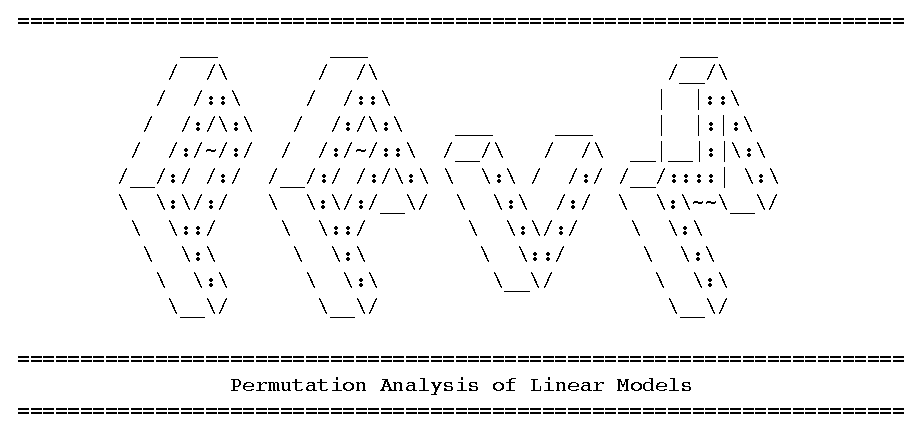
\includegraphics[width=12cm]{images/palm.eps}}
\end{center}
\caption[The proposed tests are available in \textsc{palm}.]{The permutation tests discussed and proposed in Chapters \ref{sec:perm} and \ref{sec:comb} have been made available in the tool \emph{Permutation Analysis of Linear Models} (\textsc{palm}), a text-based application that can be invoked from scripts.}
\label{fig:valor:palm}
\end{figure}

\section{Further perspectives}

The work in this thesis has already unfolded into rich consequences. The whole-block and within-block exchangeability can be nested into each other, so as to allow multi-level exchangeability blocks, a work that the author has already developed as a side-project, and that is already published \citep{Winkler2015}.

While the pycnophylactic interpolation is clearly the most appropriate way of assessing area, it is computationally demanding given the high resolution of the cortical meshes typically used, and an assessment of other, approximate methods, is necessary so as to reduce computational costs. In the same line, permutation tests are much slower than their parametric counterparts. Strategies for acceleration should to be considered if these methods are to be used for routine analysis.

Finally, the demonstration that permutation tests can be used in complex experimental designs as those considered opens up many possibilities, particularly for the analysis of multi-level \textsc{fmri} data, as well as for cases in which not all observations are present. This includes cases that currently can only be treated with linear mixed effects models, which has all the disadvantages inherent to iterative methods.
\cleardoublepage \chapter{Supplementary Material}
\label{sec:supplmat}
\setstretch{\lspac}

This dissertation includes a digital compact disc (\textsc{cd}) containing a browsable set of pages with the results of the various simulations done in Chapter~\ref{sec:comb}. The same material is available as the Supplementary Material of the paper that includes most of the content of this chapter \citep{Winkler2016}.
\cleardoublepage
\addcontentsline{toc}{chapter}{References}
\setstretch{1}
\bibliography{biblio}
\pagestyle{empty}
\cleardoublepage % ======[CURRICULUM]======
\cleardoublepage
\setstretch{1}
\vspace*{\fill}
\begin{center}
\begin{Large}
\textbf{Curriculum Vit\ae{}}
\end{Large}
\end{center}

\noindent
Anderson M.\ Winkler studied Electronics for two years before joining the Medical School at the Universidade Federal do Paran\'{a}, Curitiba, Brazil, from which he graduated in early 2005. He worked as a physician at the Centro Municipal de Urg\^{e}ncias M\'{e}dicas Boa Vista at the same time in which he studied for a Masters in Biomedical Engineering at the Universidade Tecnol\'{o}gica Federal do Paran\'{a}, Curitiba, Brazil. Upon completion, he worked for one year as Postdoctoral Associate at the Department of Psychiatry of University of Texas Health Science at San Antonio, Texas, United States, then for three years at the Department of Psychiatry of the Yale University School of Medicine. During this period he worked with brain phenotypes for imaging genetics. In 2011, he joined the Marie-Curie Initial Training Network ``Neurophysics'' programme which, with this thesis, has now reached completion.

\vspace*{\fill}

% ======[BLANK]======
%\newpage
%\pagestyle{empty}
%\vspace*{\fill}
\cleardoublepage

\end{document}          
